\chapter*{De Xi’an à Jiuzhaigou\markboth{De Xi’an à Jiuzhaigou}{}}
\section*{22 septembre 2015}
Avant de remonter sur le vélo, un peu de tourisme à Xi'an : \newline
 D'abord la fameuse armée de terre cuite à quelques dizaines de km. Il y a 3 sites à visiter, le 1er est le plus petit \newline
 \newline
\centerline{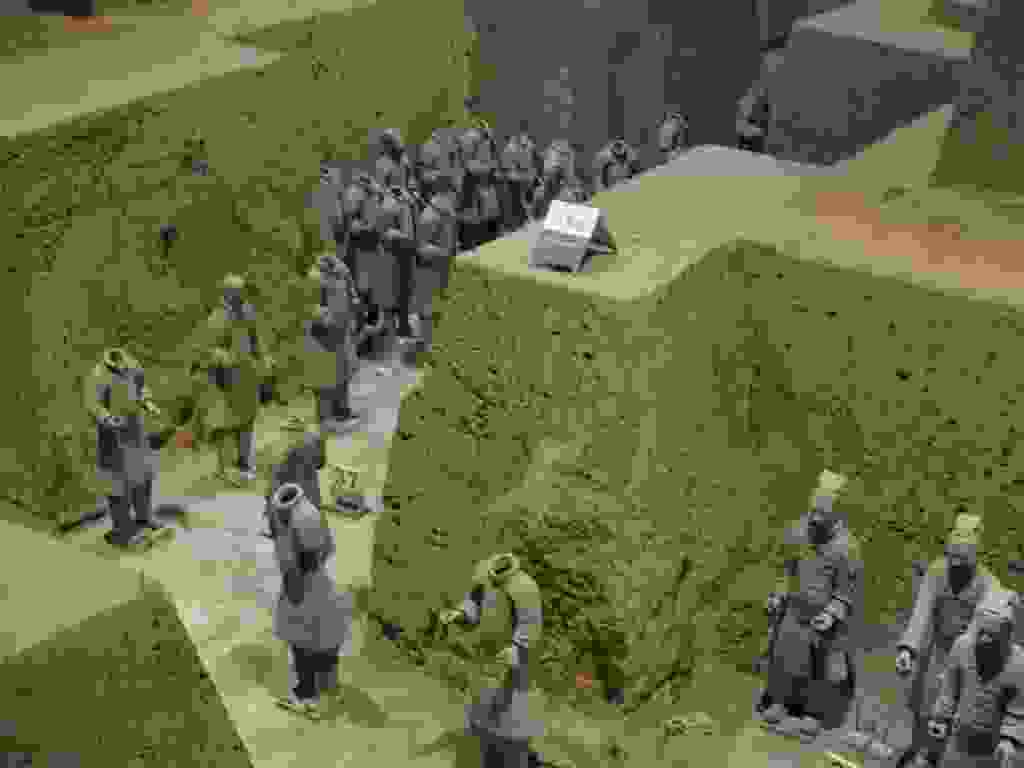
\includegraphics[width=\mywidth]{../wp-content/uploads/2015/09/wpid-wp-1442308836898-1024x768.jpg} } 
 \newline
 Le 2e est encore en cours de fouille \newline
 \newline
\centerline{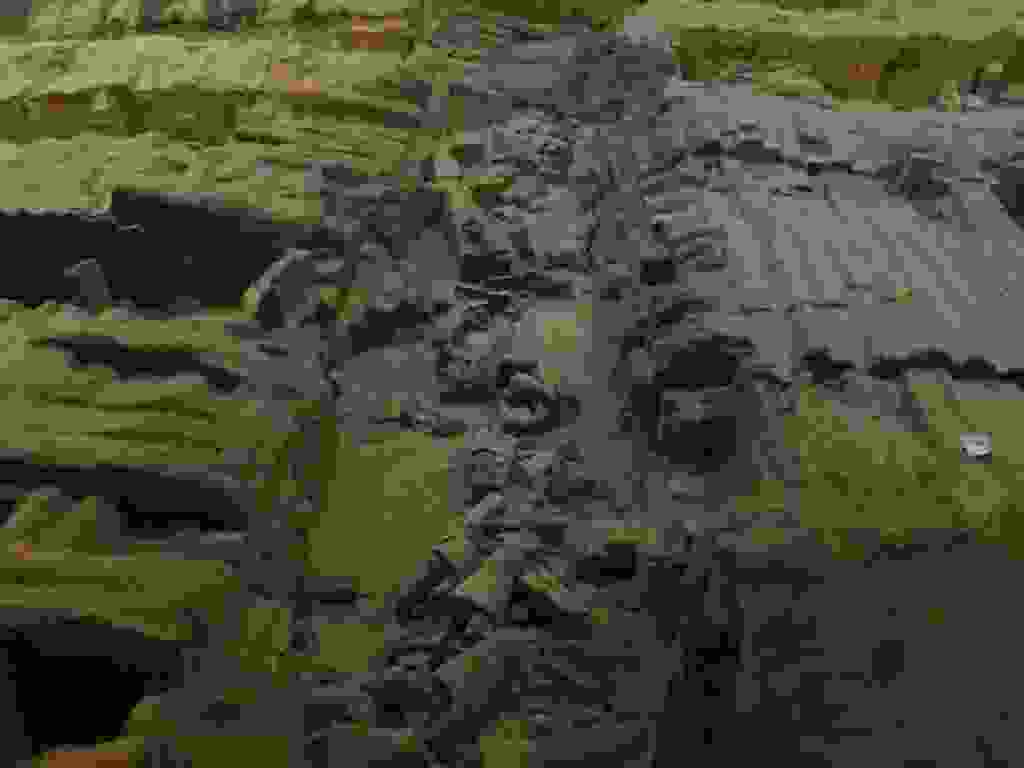
\includegraphics[width=\mywidth]{../wp-content/uploads/2015/09/wpid-wp-1442580768242-1024x768.jpg} } 
 \newline
 Enfin le dernier le plus spectaculaire \newline
 \newline
\centerline{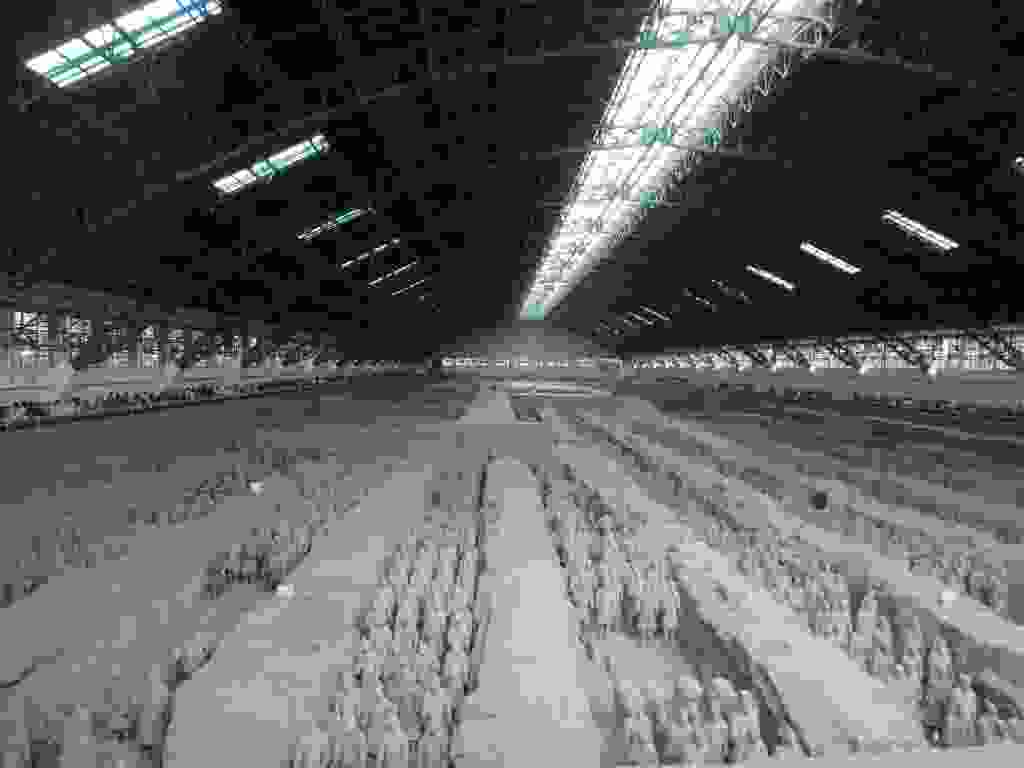
\includegraphics[width=\mywidth]{../wp-content/uploads/2015/09/wpid-wp-1442580502736-1024x768.jpg} } 
 \newline
 \newline
\centerline{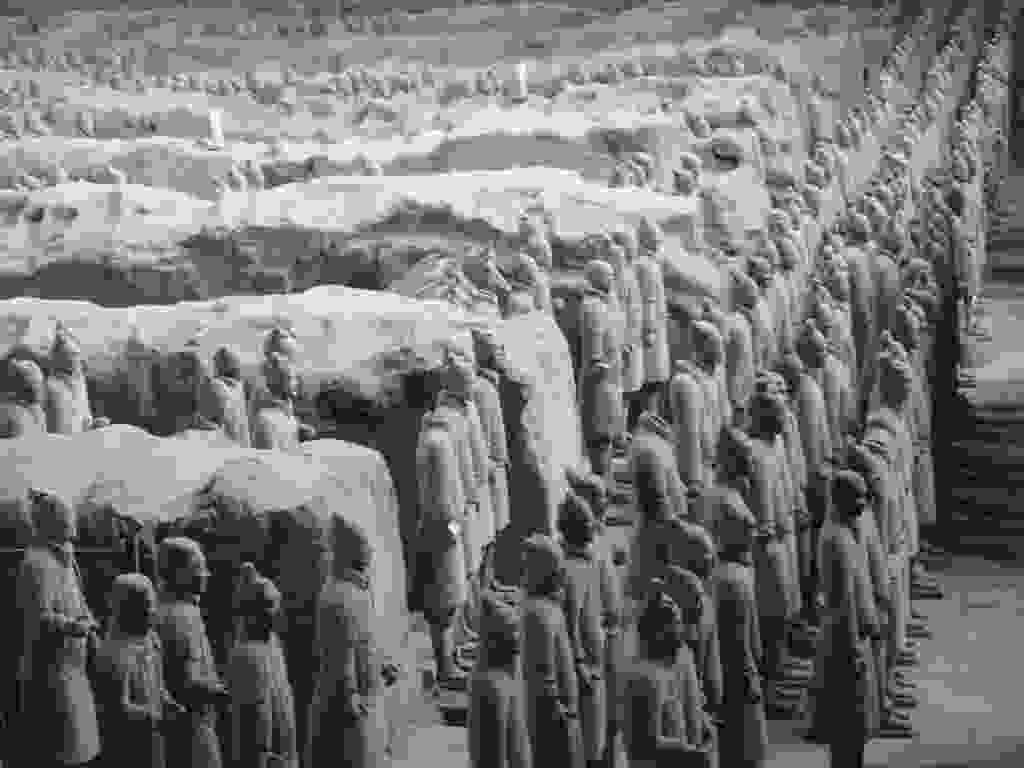
\includegraphics[width=\mywidth]{../wp-content/uploads/2015/09/wpid-wp-1442580568134-1024x768.jpg} } 
 \newline
 \newline
\centerline{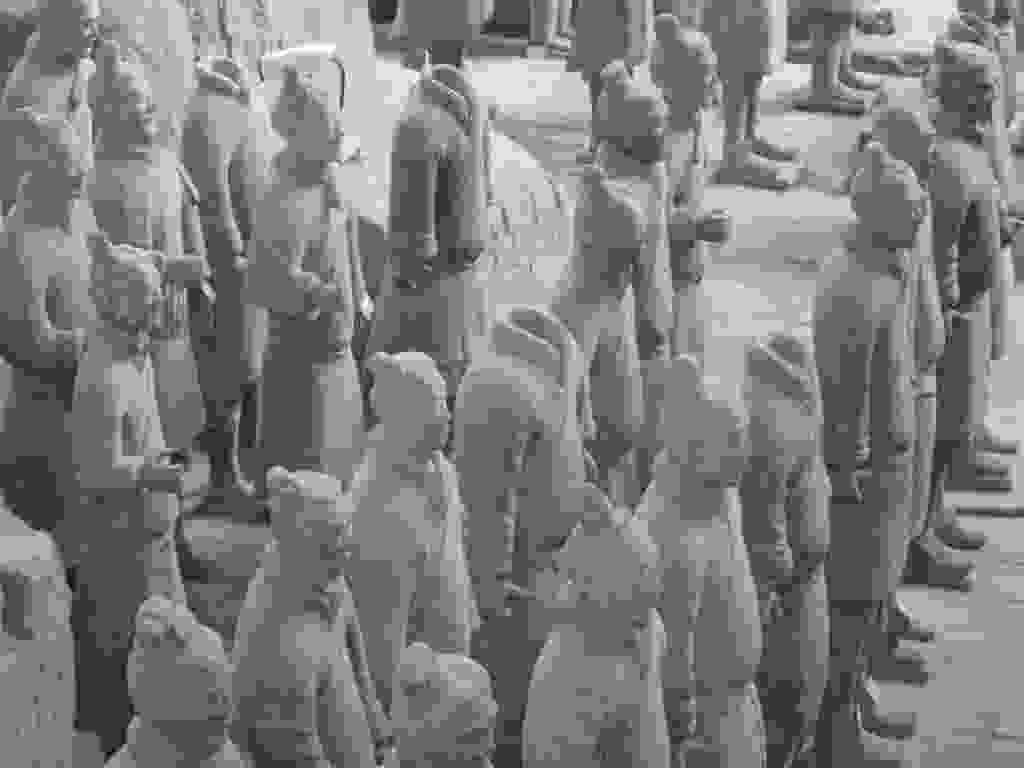
\includegraphics[width=\mywidth]{../wp-content/uploads/2015/09/wpid-wp-1442580602461-1024x768.jpg} } 
 \newline
 Des soldats en cours de restauration \newline
 \newline
\centerline{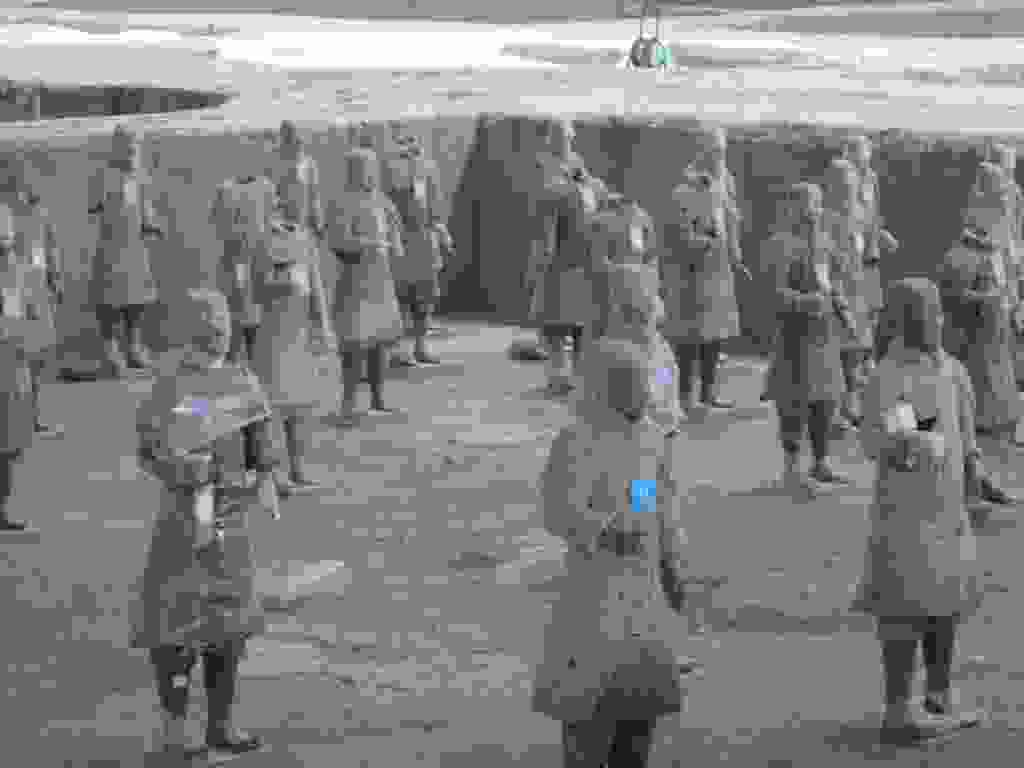
\includegraphics[width=\mywidth]{../wp-content/uploads/2015/09/wpid-wp-1442580709115-1024x768.jpg} } 
 \newline
 Xi'an est une ancienne cité chinoise situé sur la route de la soie. Le centre est entouré de remparts \newline
 \newline
\centerline{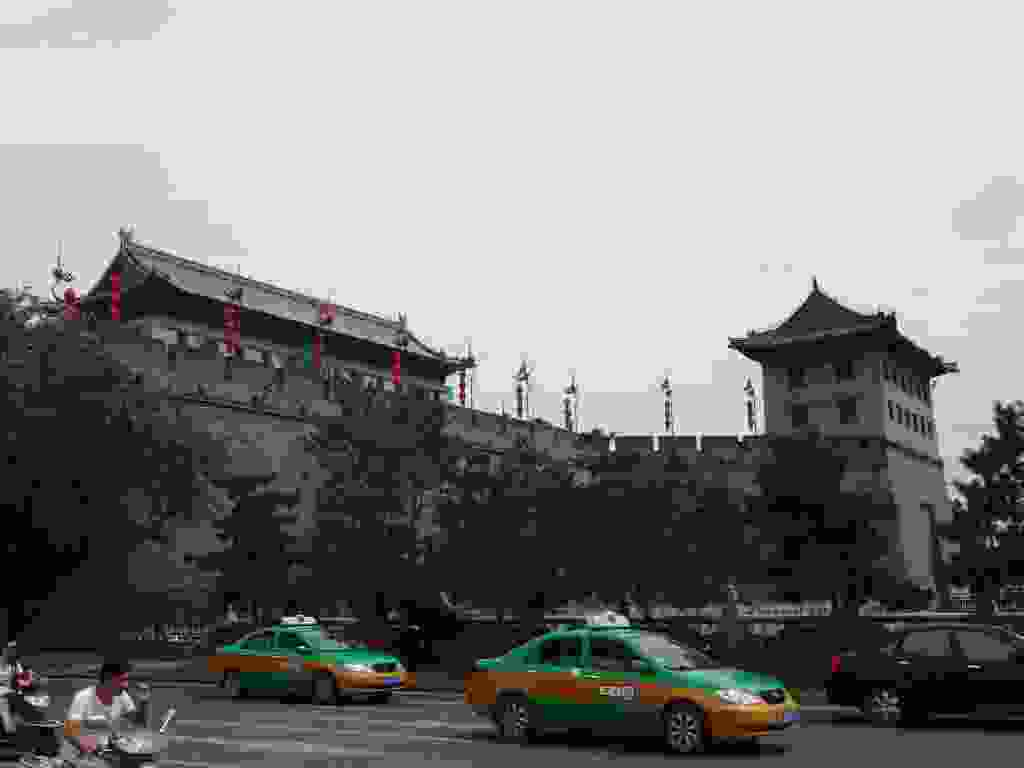
\includegraphics[width=\mywidth]{../wp-content/uploads/2015/09/wpid-wp-1442580873574-1024x768.jpg} } 
 \newline
 La grande pagode de l'oie sauvage \newline
 \newline
\centerline{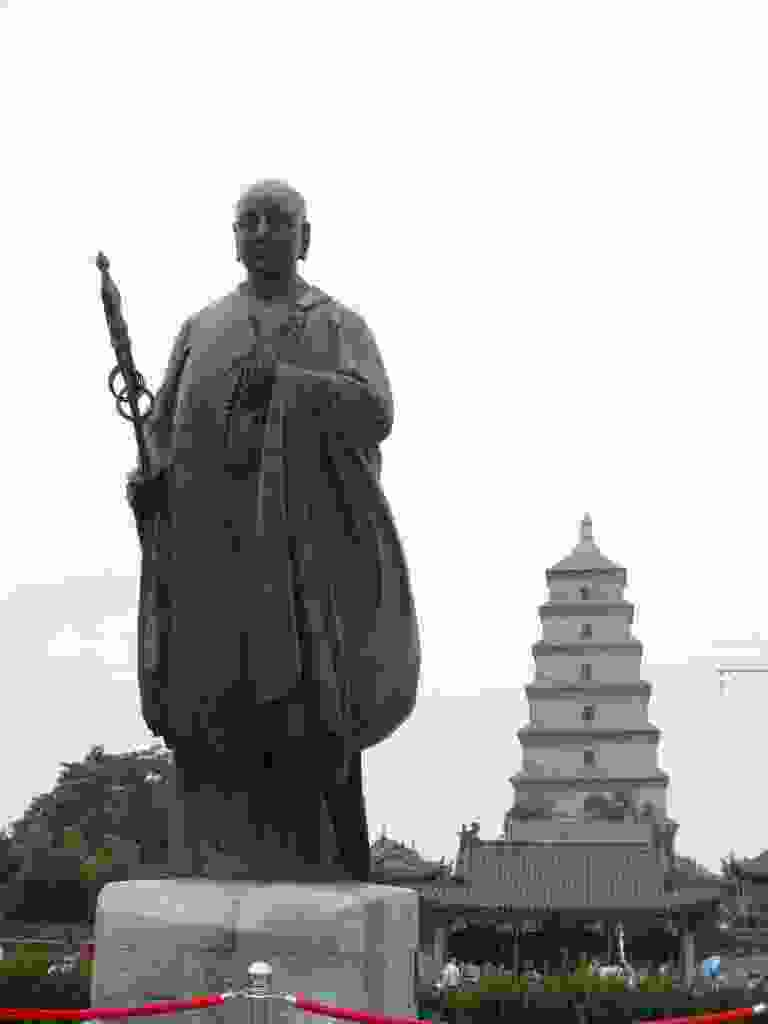
\includegraphics[width=\mywidth]{../wp-content/uploads/2015/09/wpid-wp-1442308836897-e1442739534735-768x1024.jpg} } 
 \newline
 La Bell Tower \newline
 \newline
\centerline{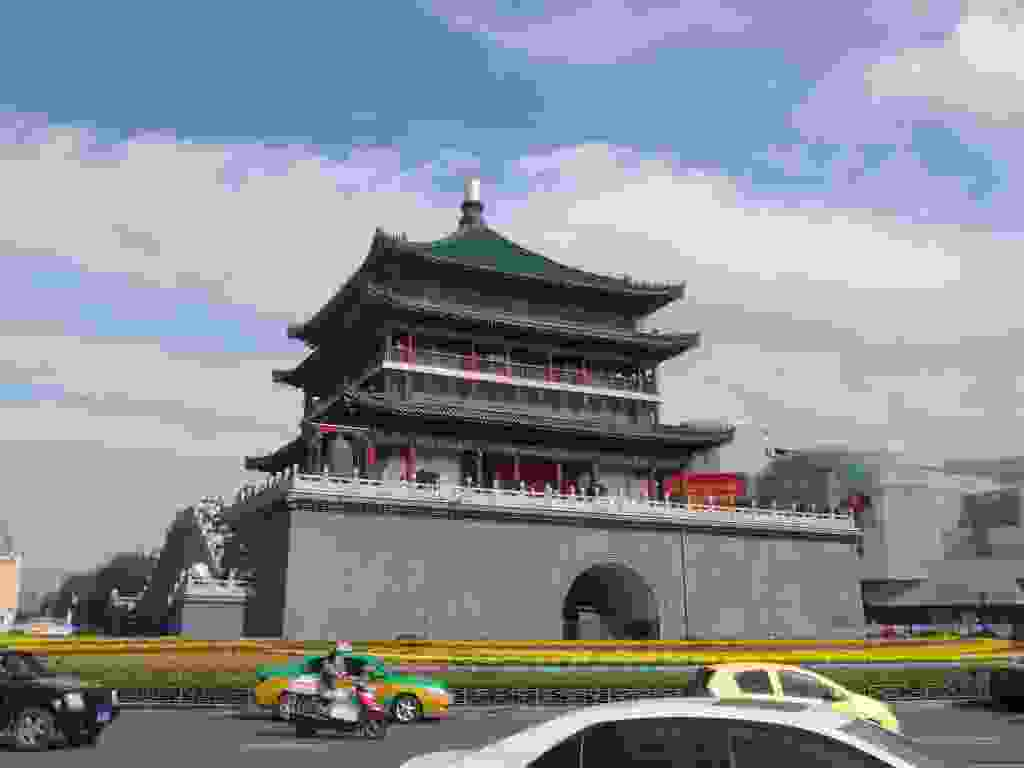
\includegraphics[width=\mywidth]{../wp-content/uploads/2015/09/wpid-wp-1442580997076-1024x768.jpg} } 
 \newline
 La Drum Tower \newline
 \newline
\centerline{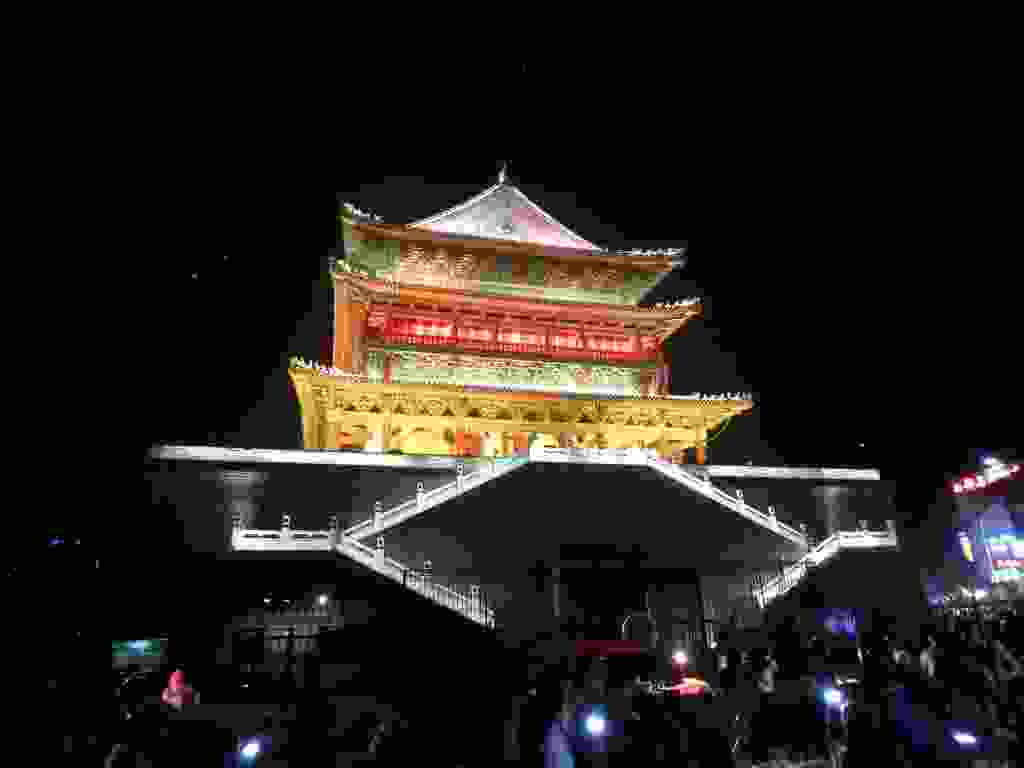
\includegraphics[width=\mywidth]{../wp-content/uploads/2015/09/wpid-wp-1442580837369-1024x768.jpg} } 
 \newline
 Le quartier musulman, très animé le jour comme la nuit \newline
 \newline
\centerline{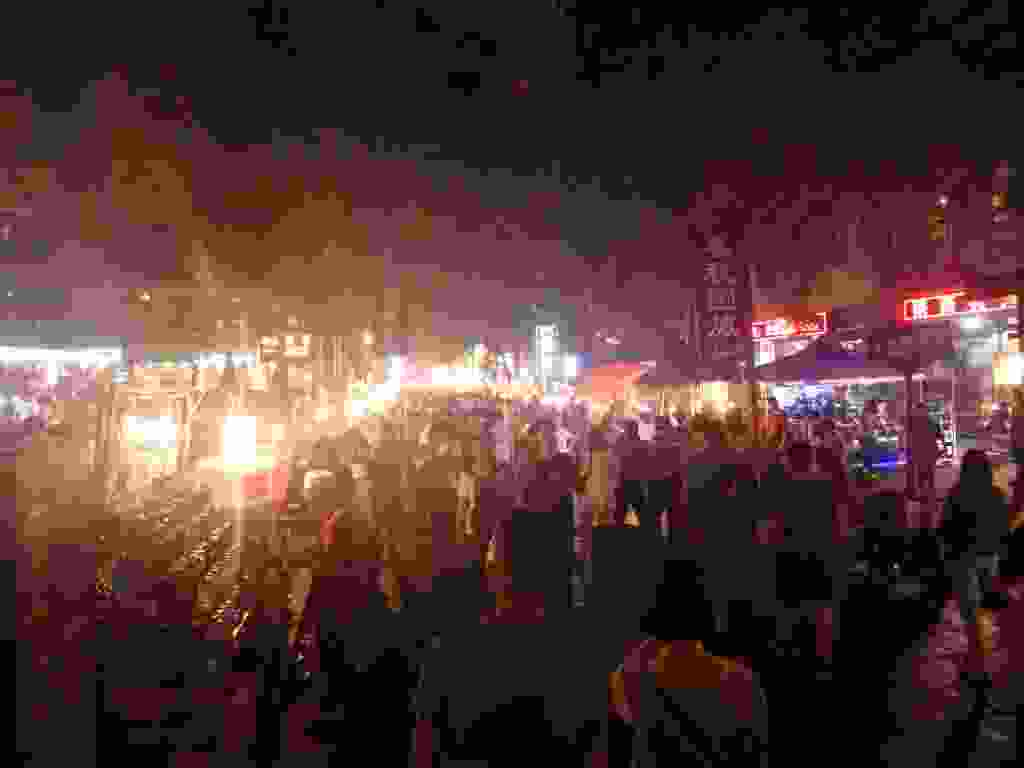
\includegraphics[width=\mywidth]{../wp-content/uploads/2015/09/P9046684-1024x768.jpg} } 
 \newline
 \newline
\centerline{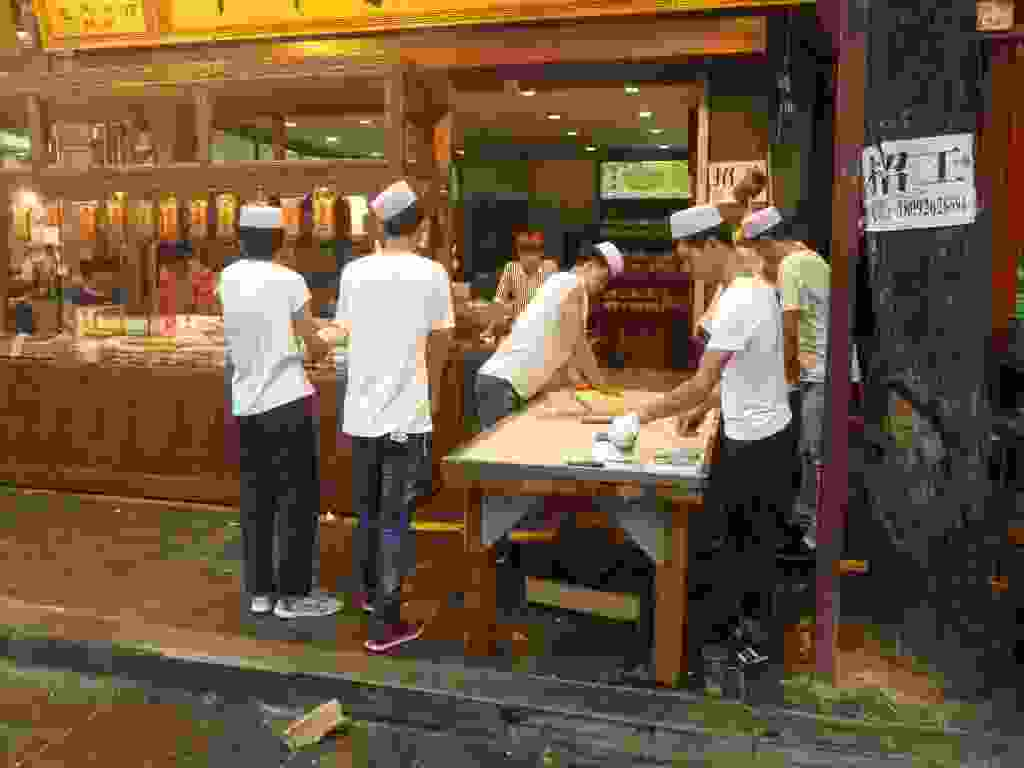
\includegraphics[width=\mywidth]{../wp-content/uploads/2015/09/wpid-wp-1442581025952-1024x768.jpg} } 
 \newline
 Dans les restaurants, les spécialités sont différent types de nouilles faites maison avec sauce épicée et souvent viande d'agneau \newline
 \newline
\centerline{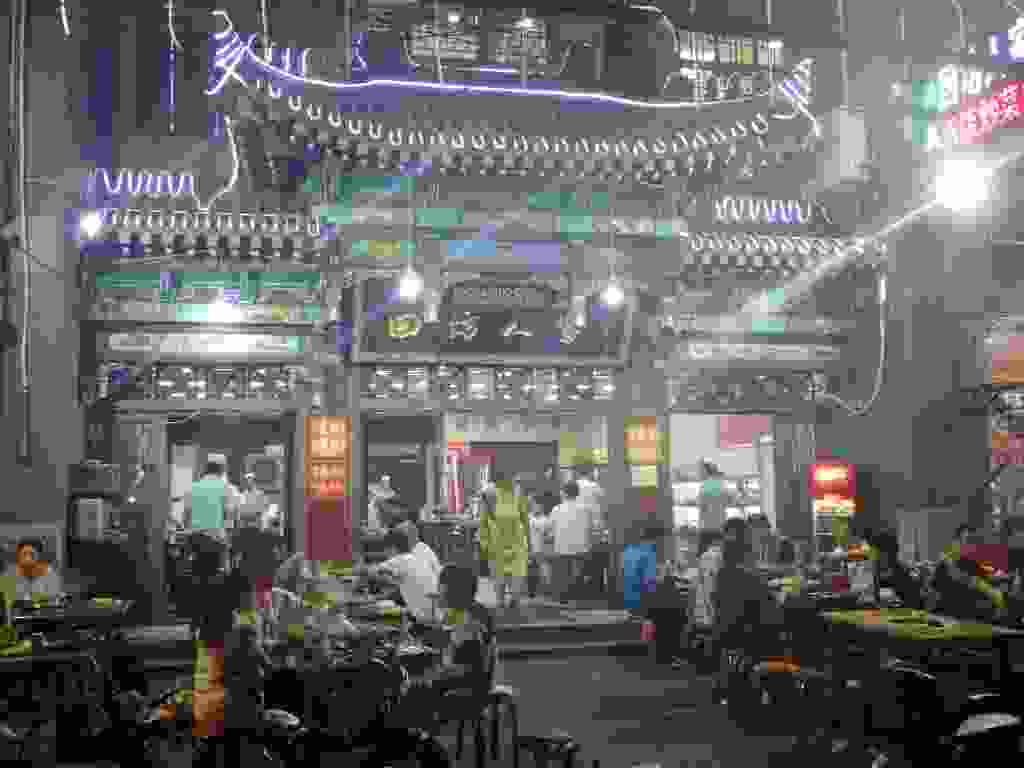
\includegraphics[width=\mywidth]{../wp-content/uploads/2015/09/P9046679-1024x768.jpg} } 
 \newline
 \newline
\centerline{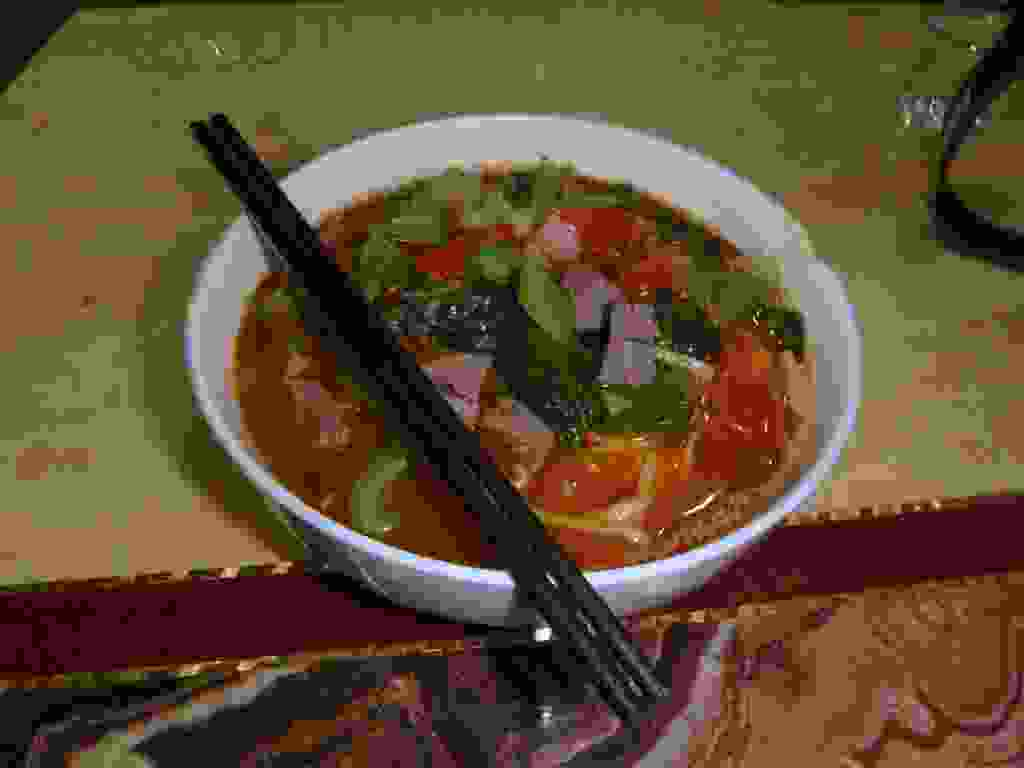
\includegraphics[width=\mywidth]{../wp-content/uploads/2015/09/P9046678-1024x768.jpg} } 
 \newline
 La grande mosquée \newline
 \newline
\centerline{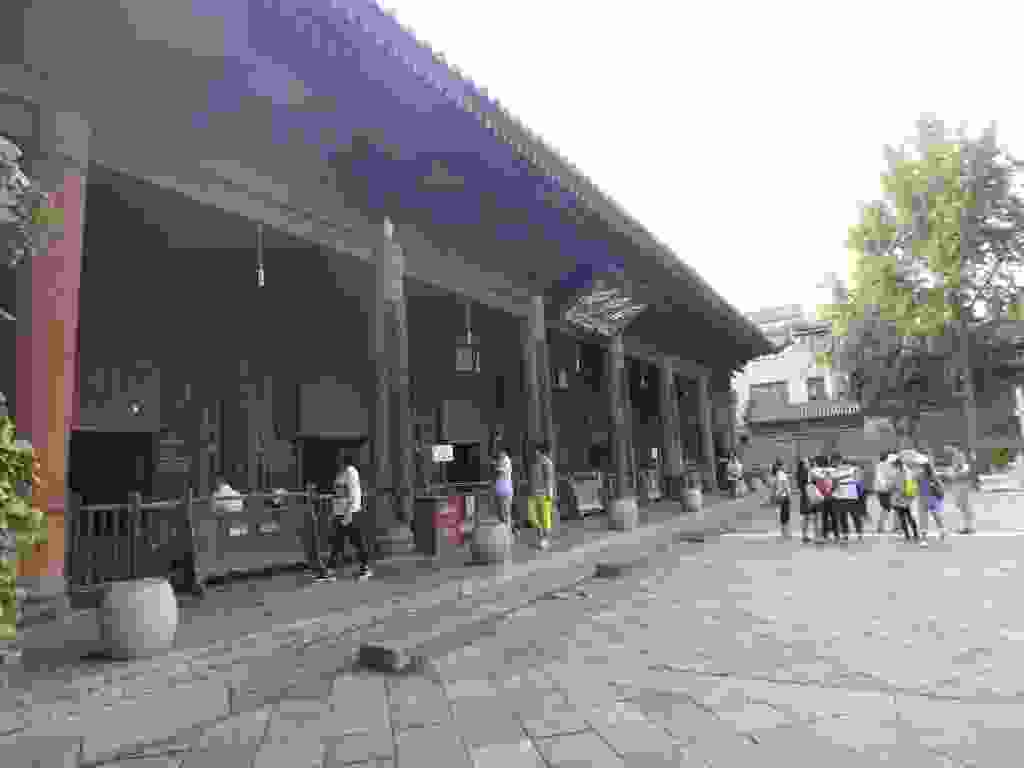
\includegraphics[width=\mywidth]{../wp-content/uploads/2015/09/wpid-wp-1442581072476-1024x768.jpg} } 
 \newline
 \newline
\centerline{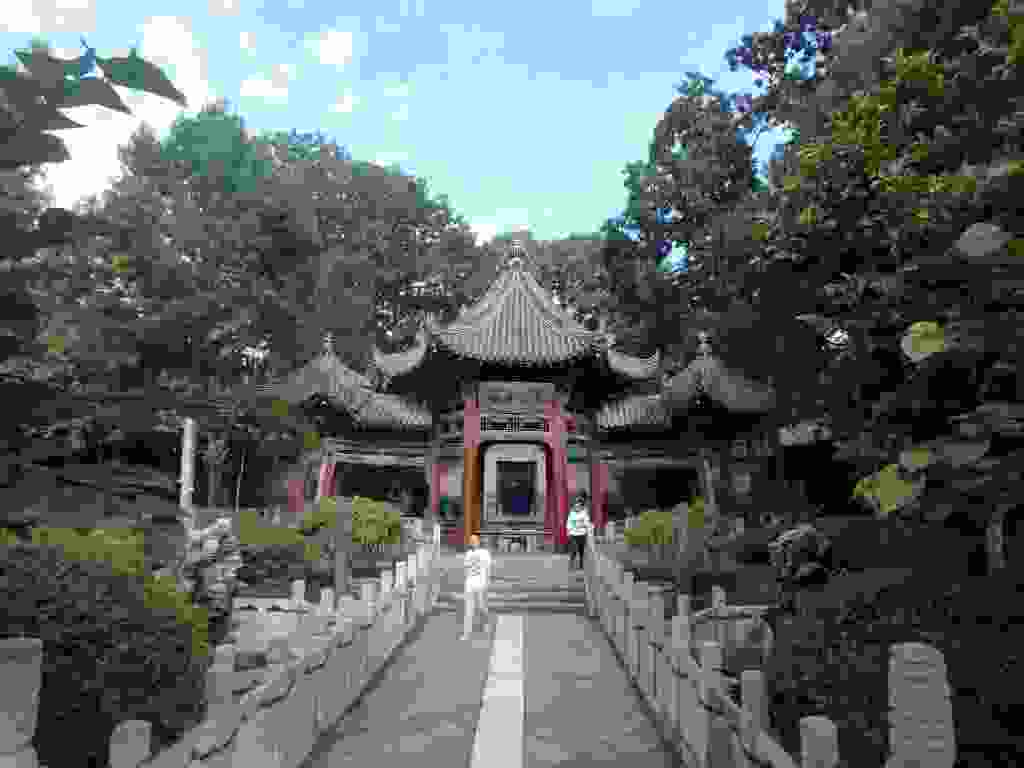
\includegraphics[width=\mywidth]{../wp-content/uploads/2015/09/wpid-wp-1442581100743-1024x768.jpg} } 
 \newline
 Le temple Wolong, je vois les moines en train de chanter \newline
 \newline
\centerline{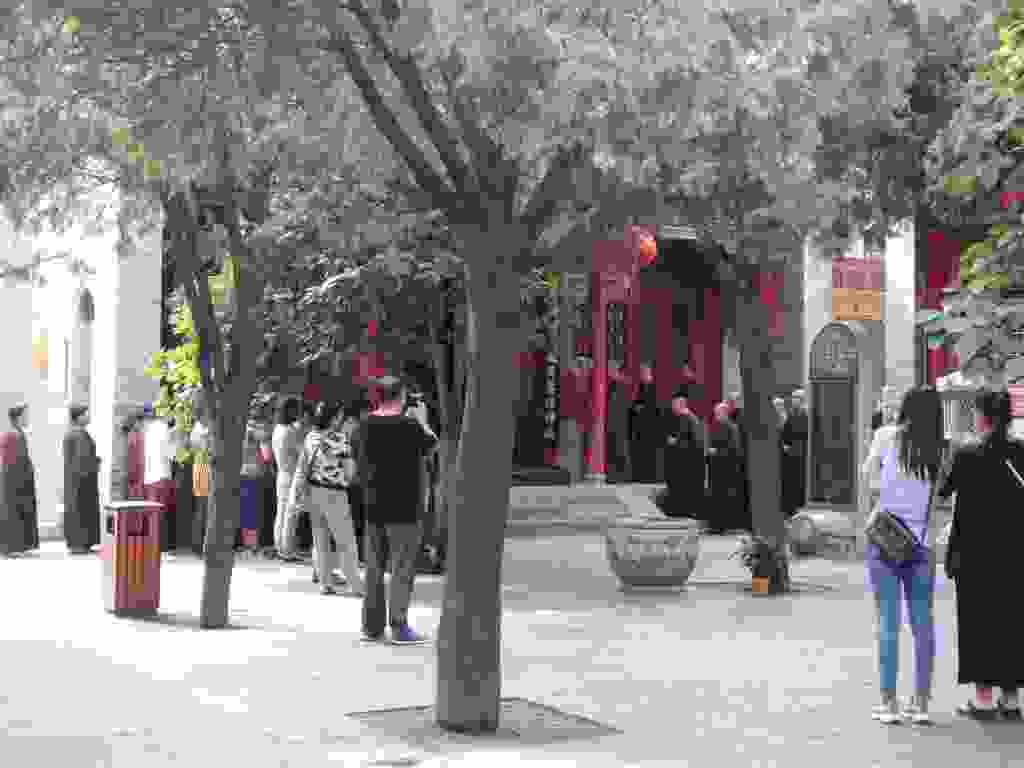
\includegraphics[width=\mywidth]{../wp-content/uploads/2015/09/wpid-wp-1442308836939-1024x768.jpg} } 
 \newline
 Je quitte Xi'an vers l'ouest pour 9 jours de vélo jusqu'à Jiuzhaigou. Premières impressions : ça roule n'importe comment mais assez lentement, j'ai le temps de voir venir \newline
 Pour sortir de la ville, quelques pistes cyclables utilisées par les scooters électriques et les velib \newline
 \newline
\centerline{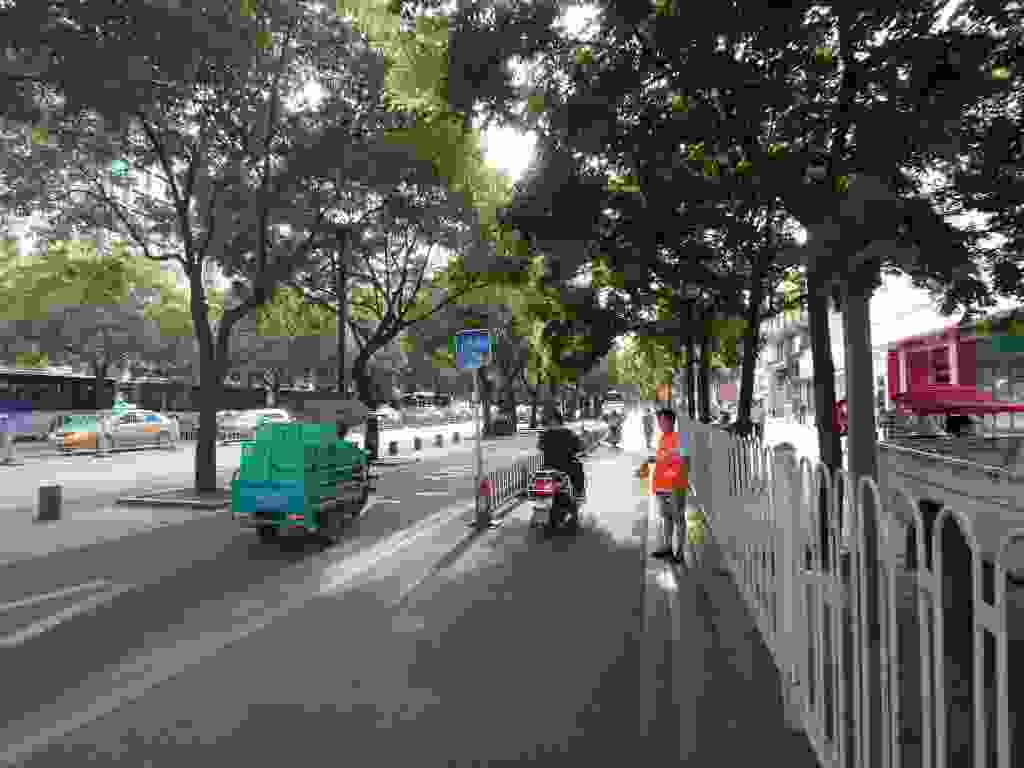
\includegraphics[width=\mywidth]{../wp-content/uploads/2015/09/wpid-wp-1442581159940-1024x768.jpg} } 
 \newline
 \newline
\centerline{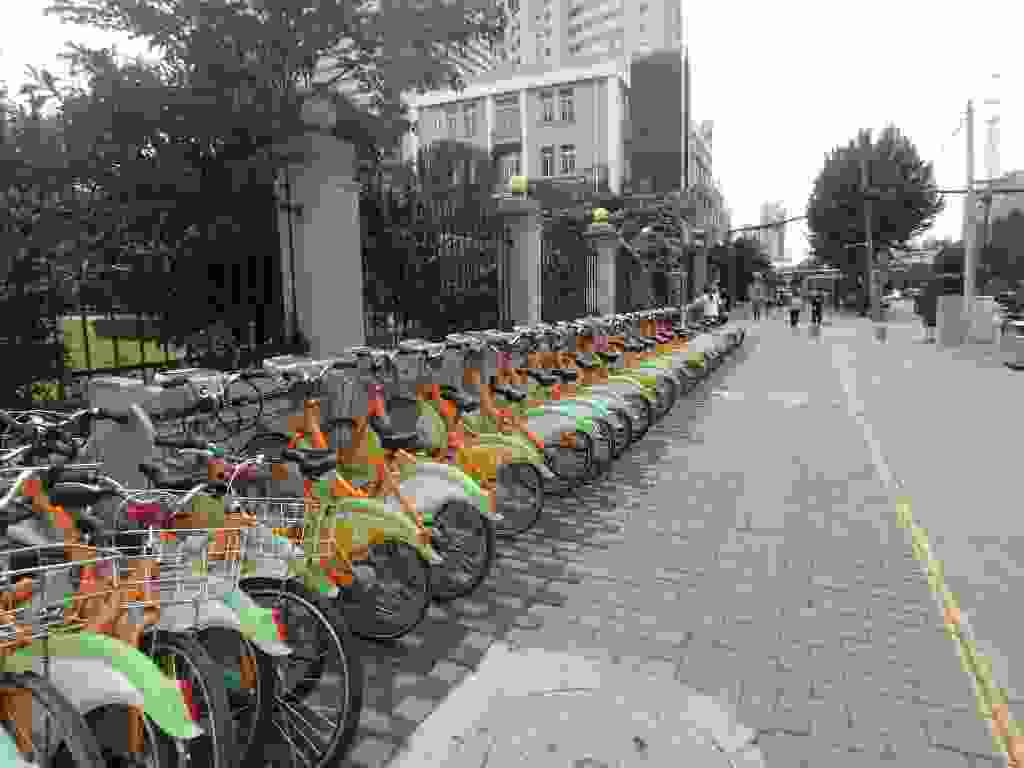
\includegraphics[width=\mywidth]{../wp-content/uploads/2015/09/wpid-wp-1442308836863-1024x768.jpg} } 
 \newline
 2 jours de plat pour commencer, au milieu des champs et des usines \newline
 \newline
\centerline{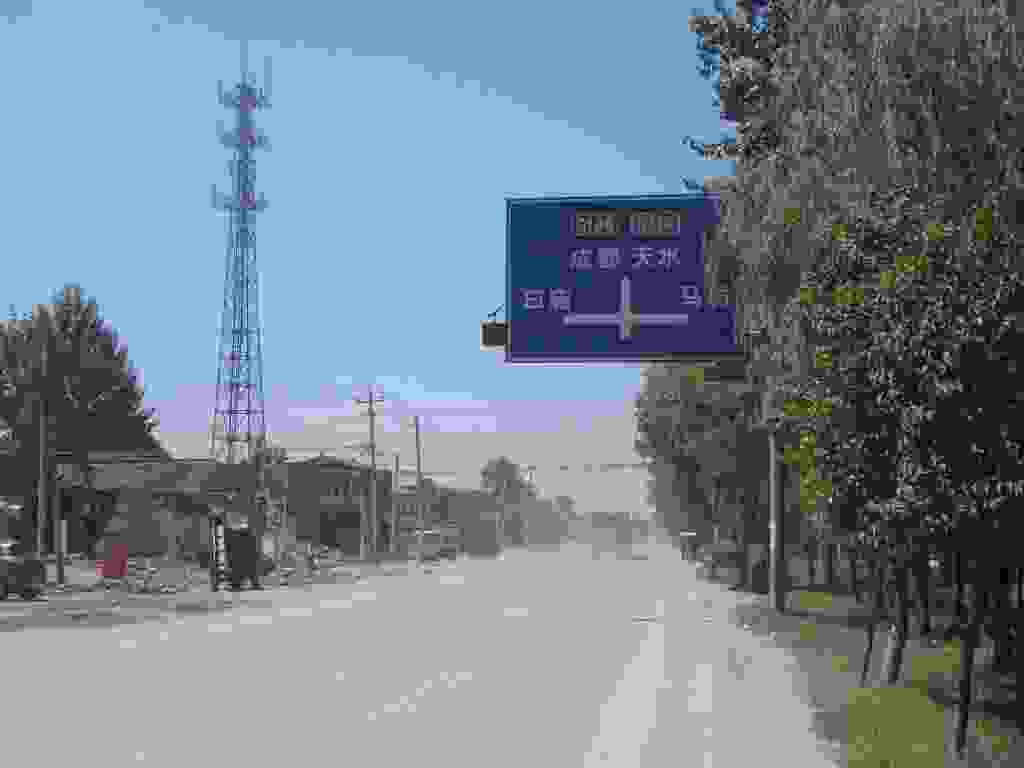
\includegraphics[width=\mywidth]{../wp-content/uploads/2015/09/wpid-p9066732-1024x768.jpg} } 
 \newline
 Puis les cols s'enchaînent ainsi que 3 jours de pluie, quelques rares moments pour apprécier le paysage \newline
 \newline
\centerline{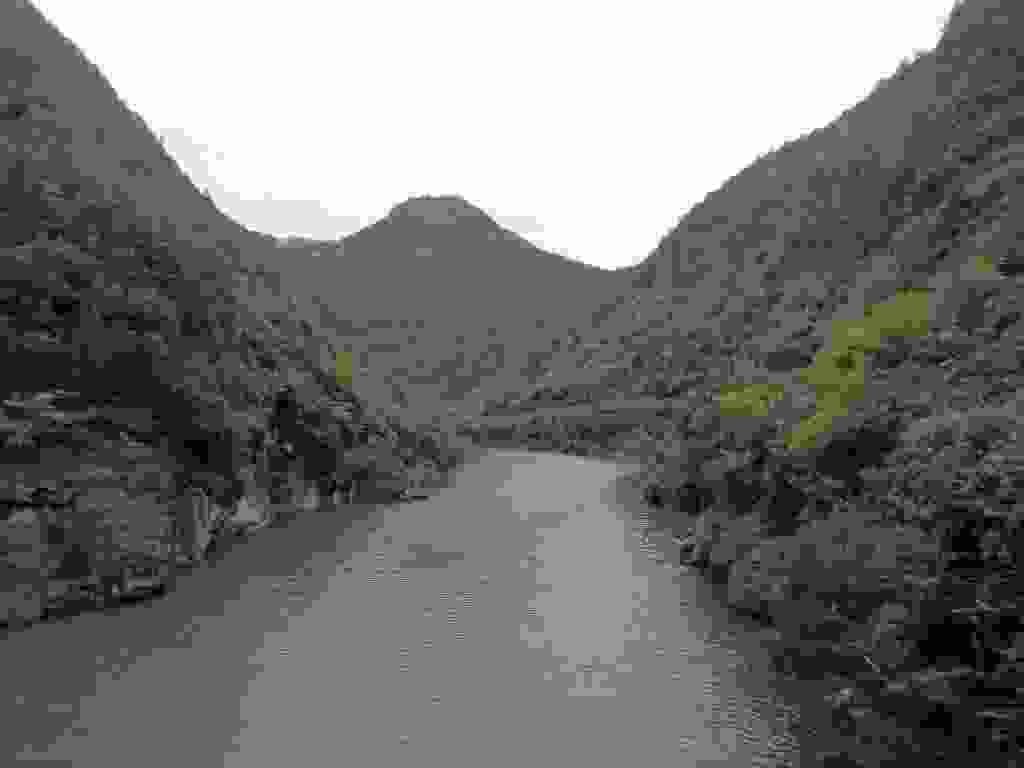
\includegraphics[width=\mywidth]{../wp-content/uploads/2015/09/wpid-p9096768-1024x768.jpg} } 
 \newline
 \newline
\centerline{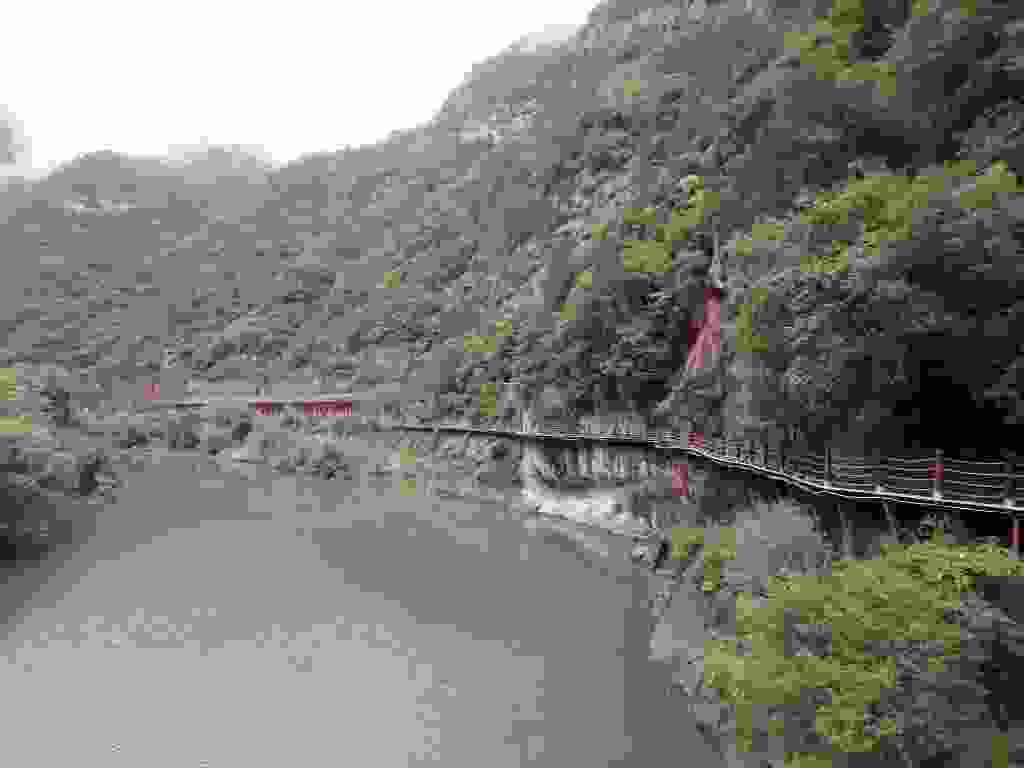
\includegraphics[width=\mywidth]{../wp-content/uploads/2015/09/wpid-p9096769-1024x768.jpg} } 
 \newline
 \newline
\centerline{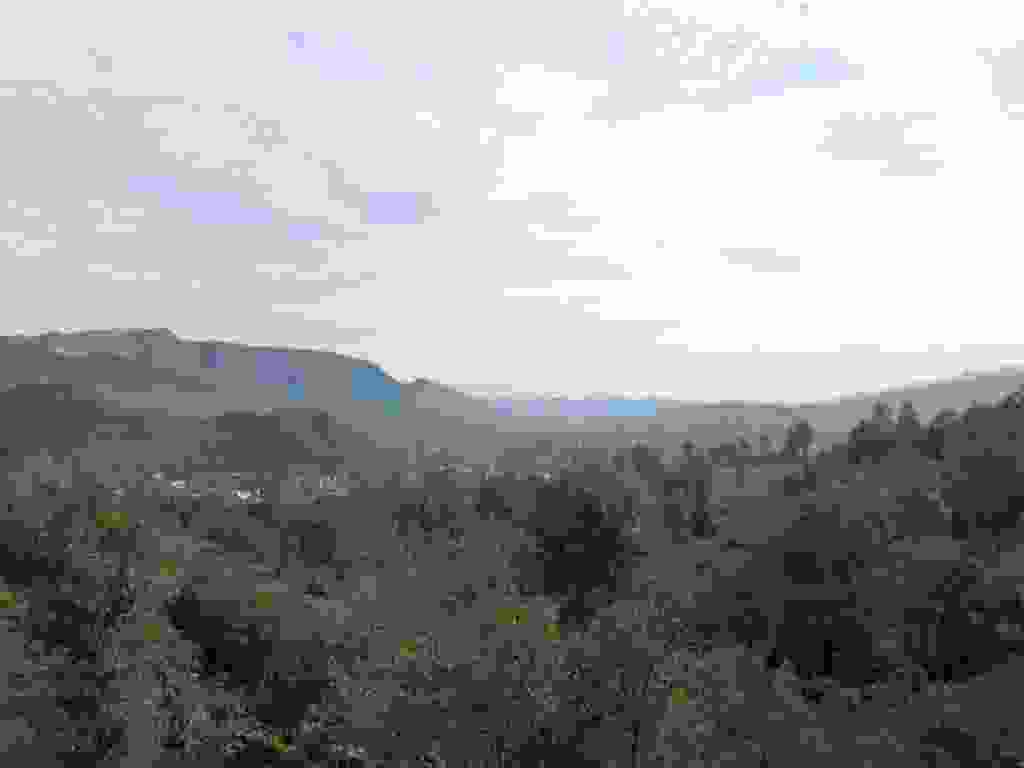
\includegraphics[width=\mywidth]{../wp-content/uploads/2015/09/wpid-p9116786-1024x768.jpg} } 
 \newline
 \newline
\centerline{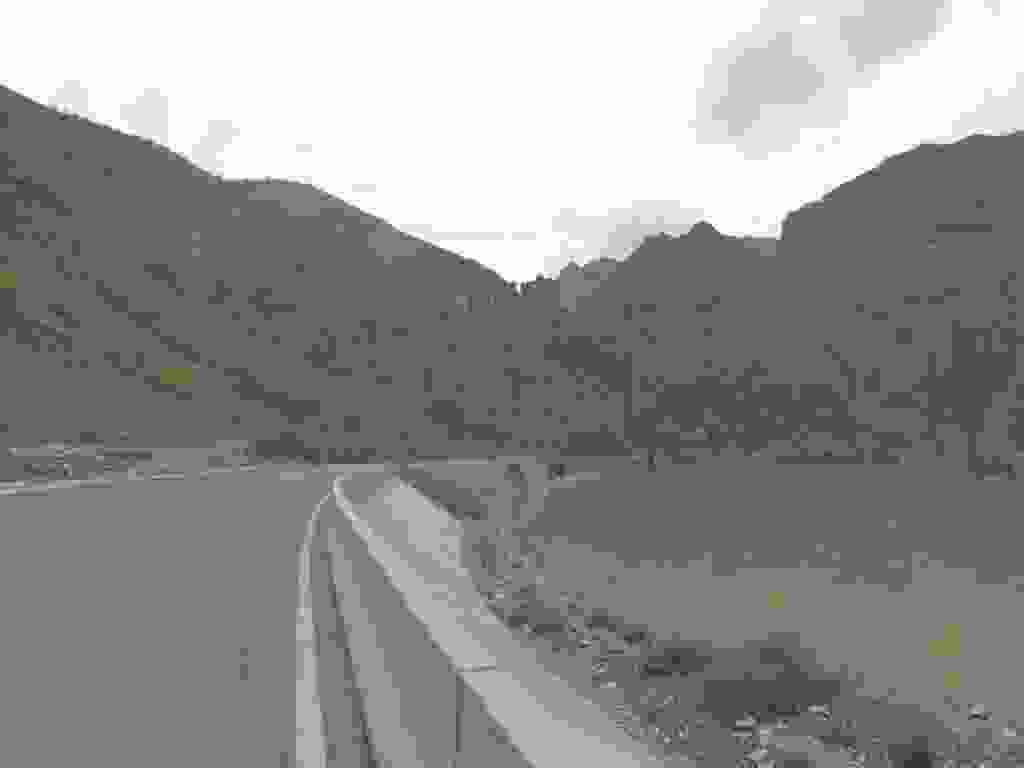
\includegraphics[width=\mywidth]{../wp-content/uploads/2015/09/wpid-p9126807-1024x768.jpg} } 
 \newline
 J'alterne camping et hôtel, pas facile à identifier dans les villages \newline
 \newline
\centerline{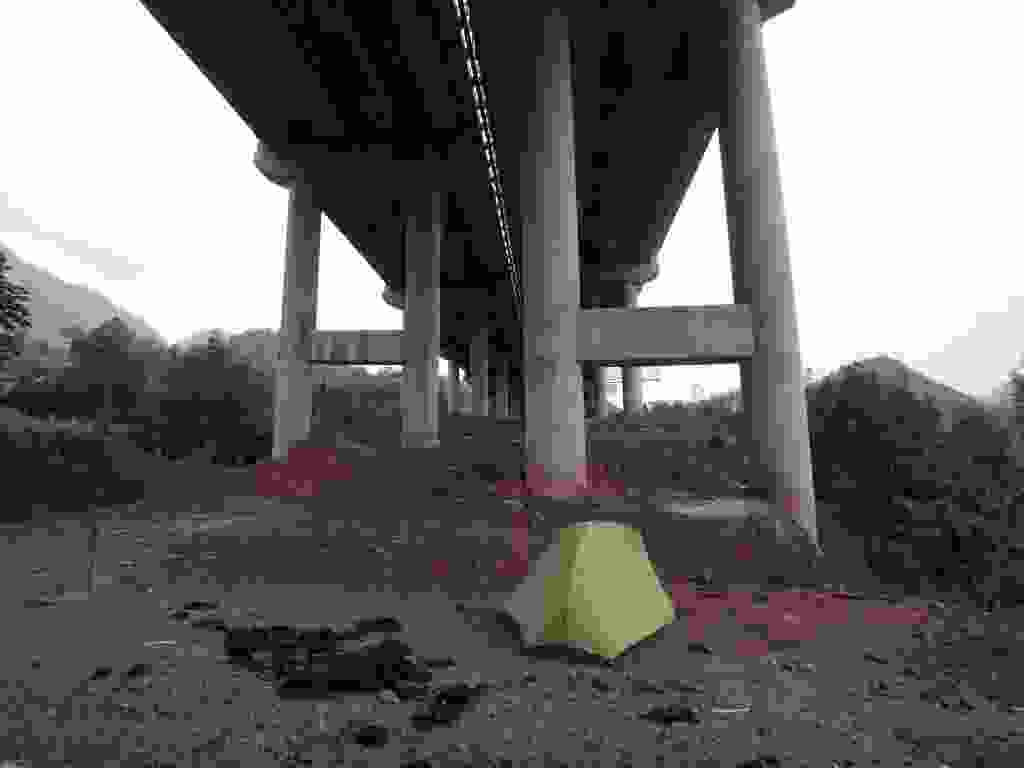
\includegraphics[width=\mywidth]{../wp-content/uploads/2015/09/wpid-p9106784-1024x768.jpg} } 
 \newline
 Les villes sont modernes avec des grands immeubles en construction partout \newline
 \newline
\centerline{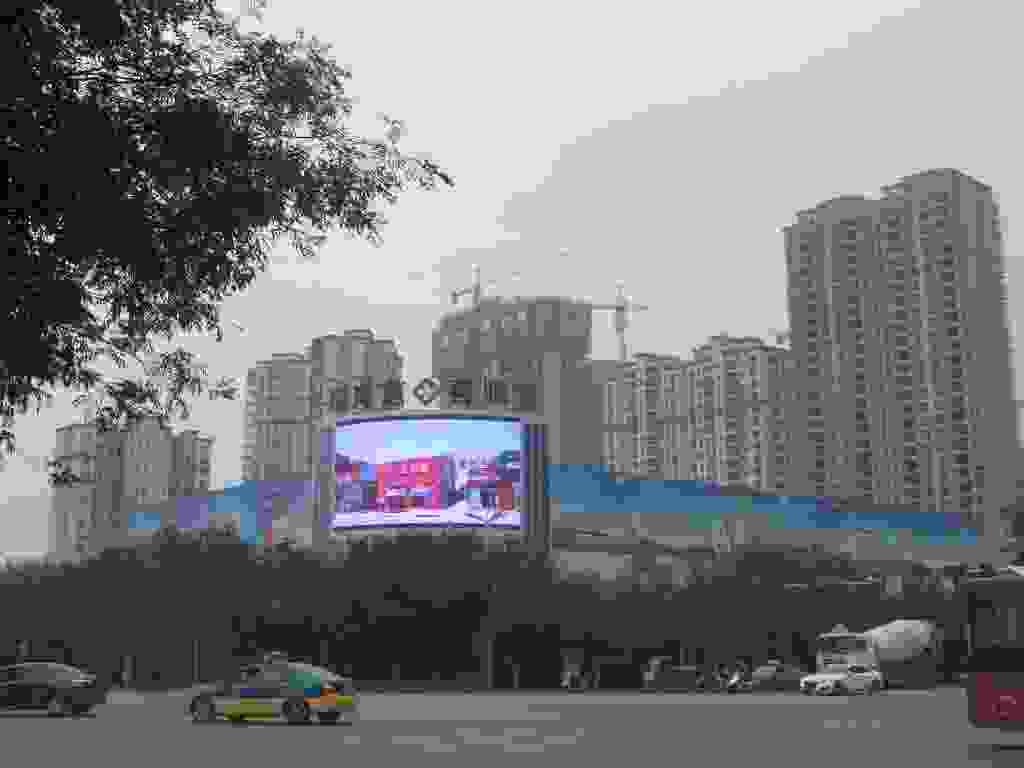
\includegraphics[width=\mywidth]{../wp-content/uploads/2015/09/P9076744-1024x768.jpg} } 
 \newline
 \newline
\centerline{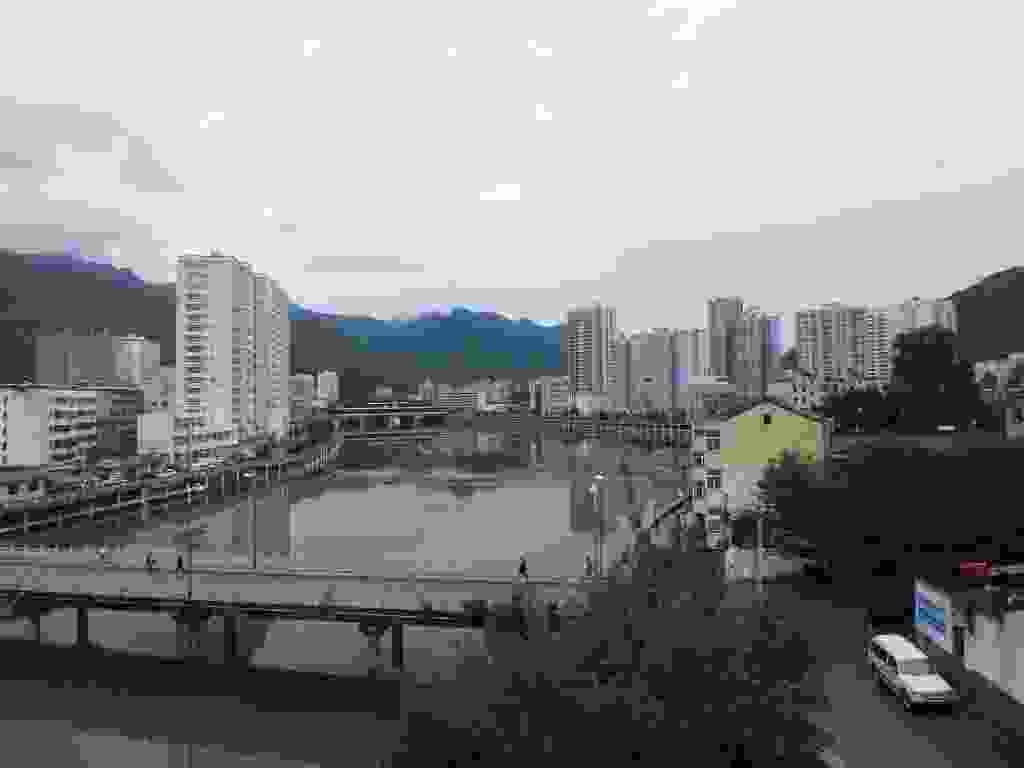
\includegraphics[width=\mywidth]{../wp-content/uploads/2015/09/wpid-p9096761-1024x768.jpg} } 
 \newline
 \newline
\centerline{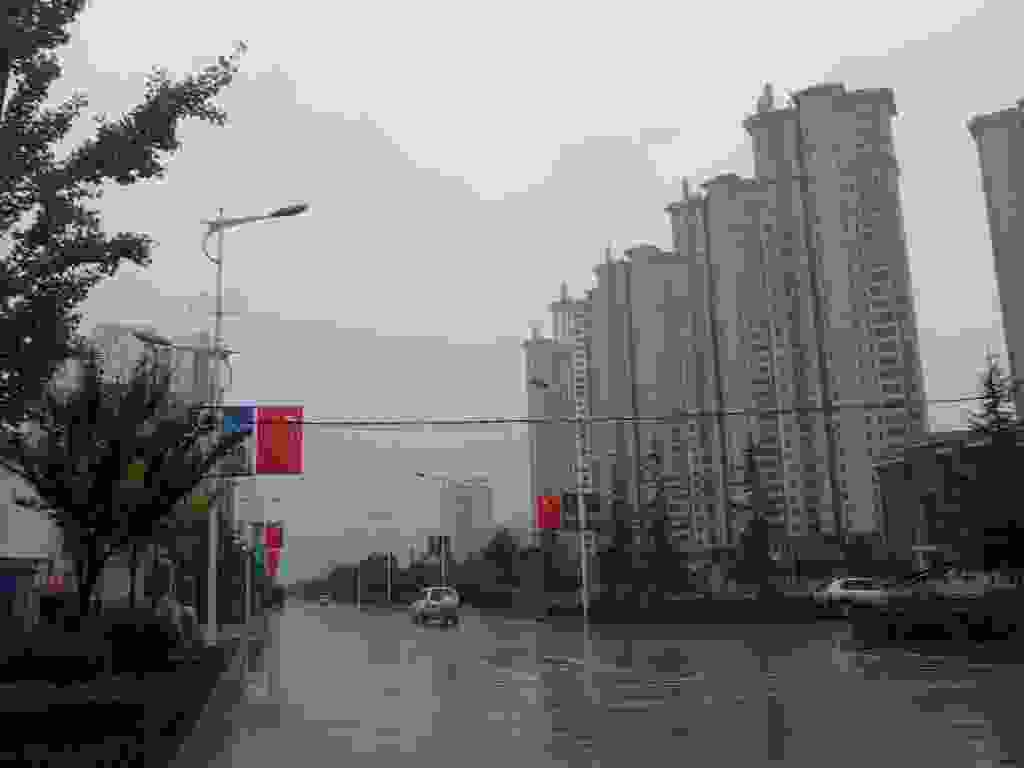
\includegraphics[width=\mywidth]{../wp-content/uploads/2015/09/P9106779-1024x768.jpg} } 
 \newline
 Les villages semblent beaucoup moins développés \newline
 \newline
\centerline{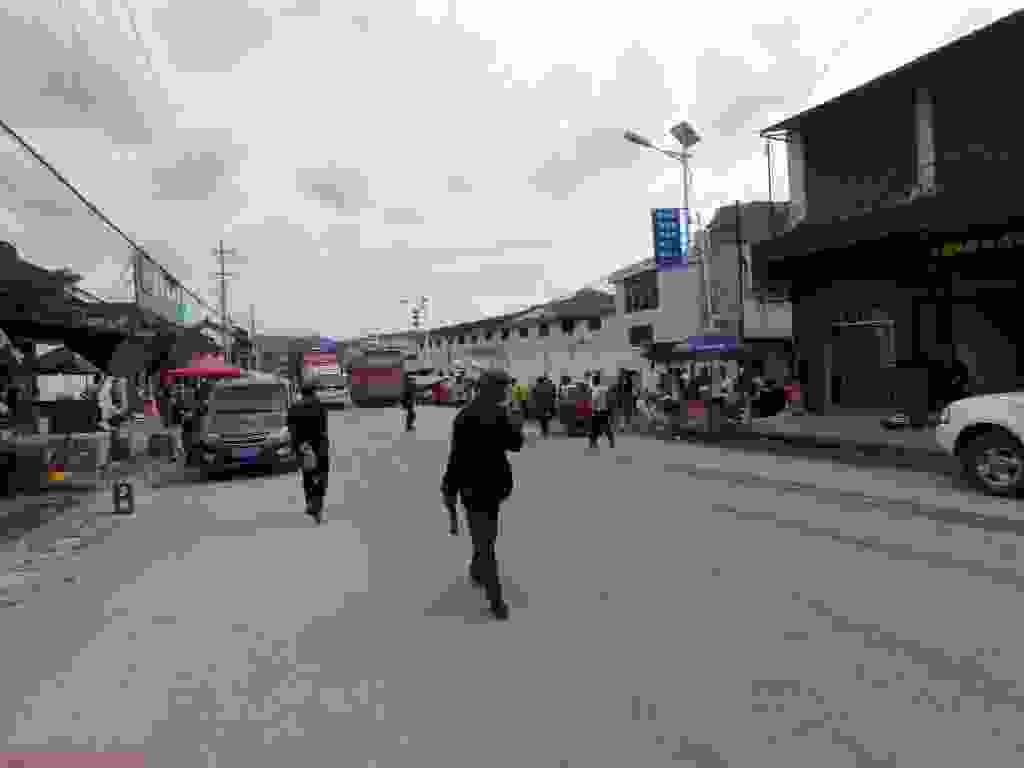
\includegraphics[width=\mywidth]{../wp-content/uploads/2015/09/wpid-p9116788-1024x768.jpg} } 
 \newline
 Plusieurs temples le long de la route \newline
 \newline
\centerline{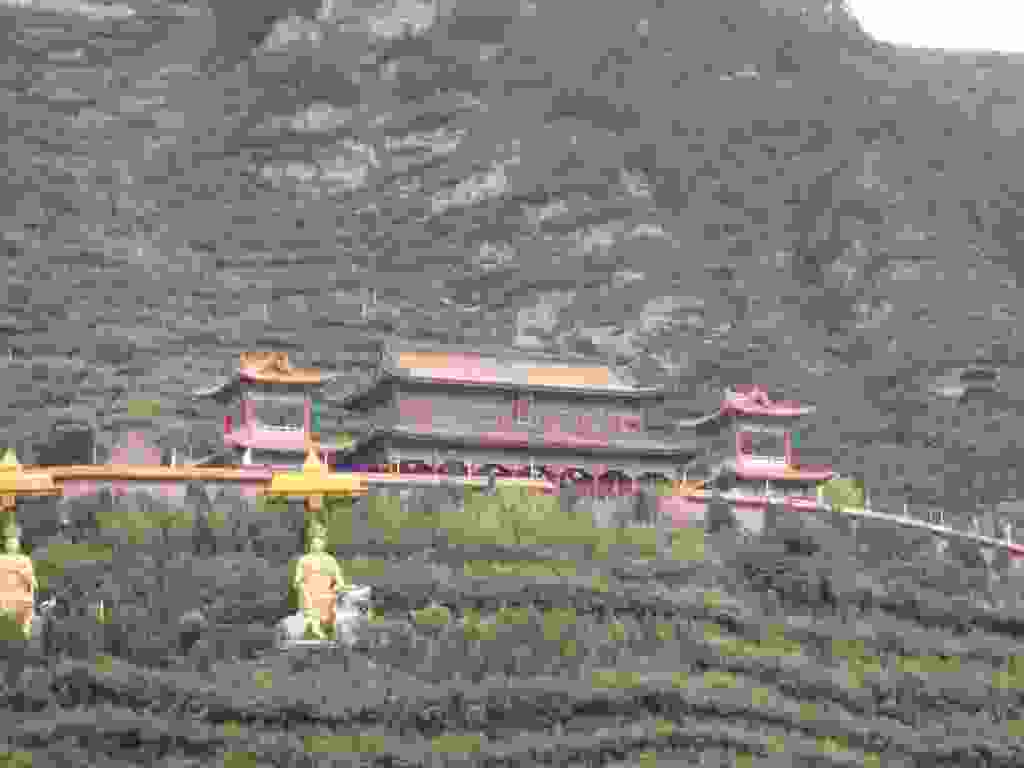
\includegraphics[width=\mywidth]{../wp-content/uploads/2015/09/wpid-wp-1442581295173-1024x768.jpg} } 
 \newline
 \newline
\centerline{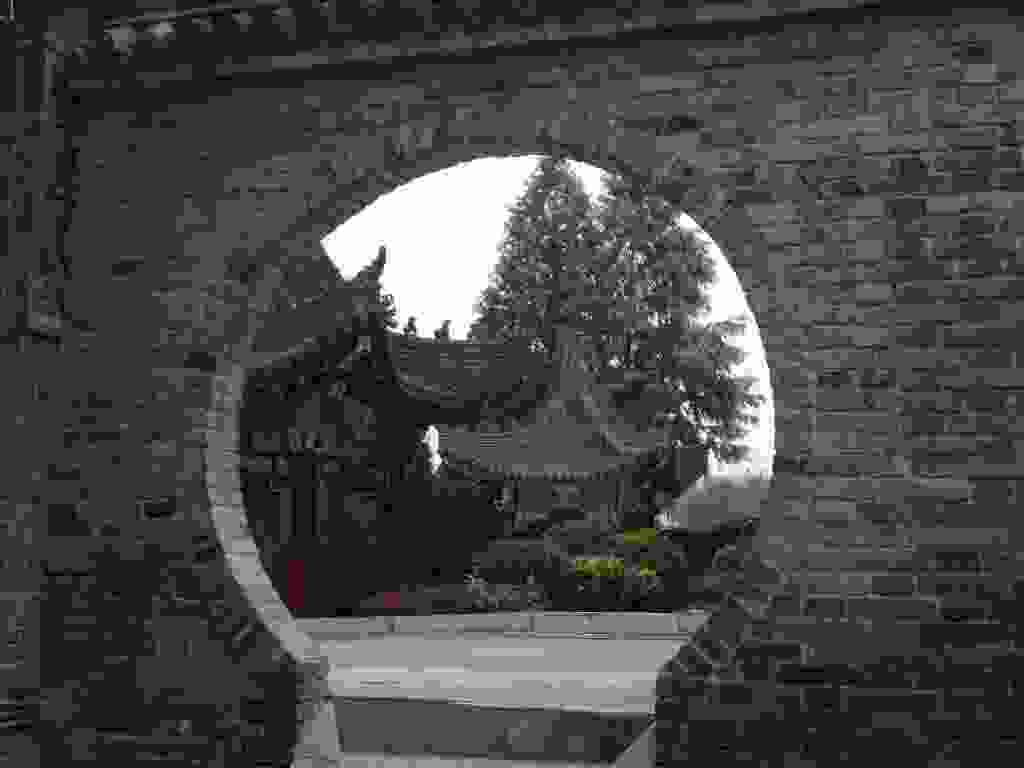
\includegraphics[width=\mywidth]{../wp-content/uploads/2015/09/P9076737-1024x768.jpg} } 
 \newline
 Peu de trafic sur certaines portions qui longent l'autoroute toute neuve \newline
 \newline
\centerline{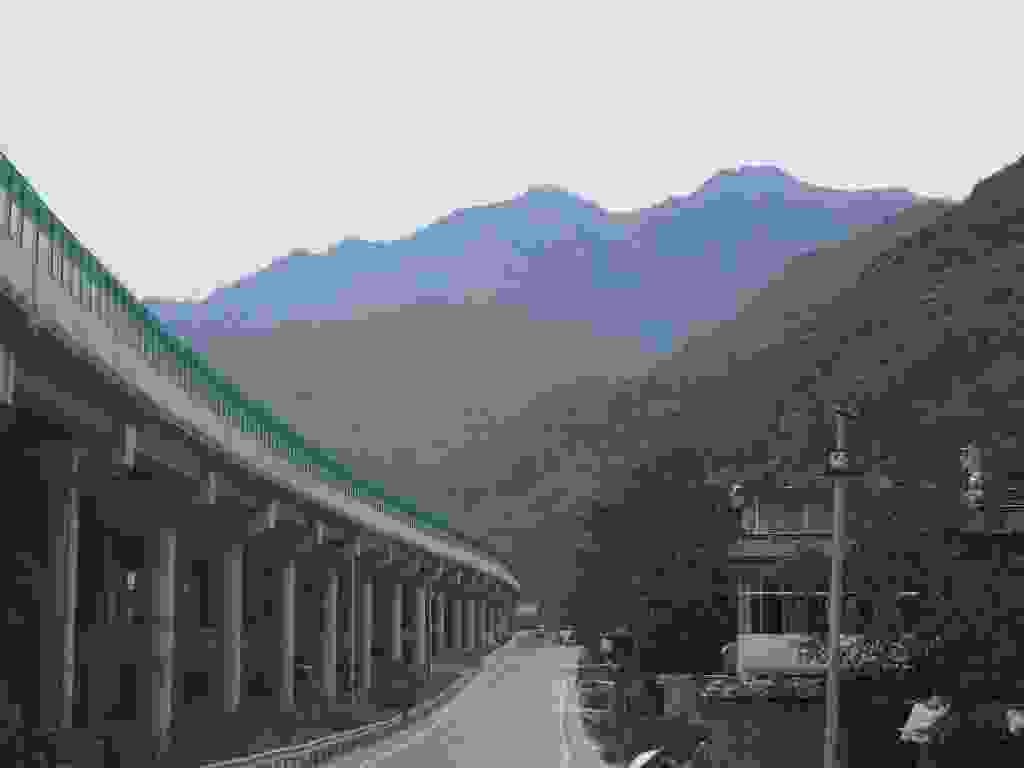
\includegraphics[width=\mywidth]{../wp-content/uploads/2015/09/wpid-p9116795-1024x768.jpg} } 
 \newline
 Je m'arrête dans un village, un homme m'aide à chercher un hotel puis finalement m'invite à passer la nuit chez lui \newline
 \newline
\centerline{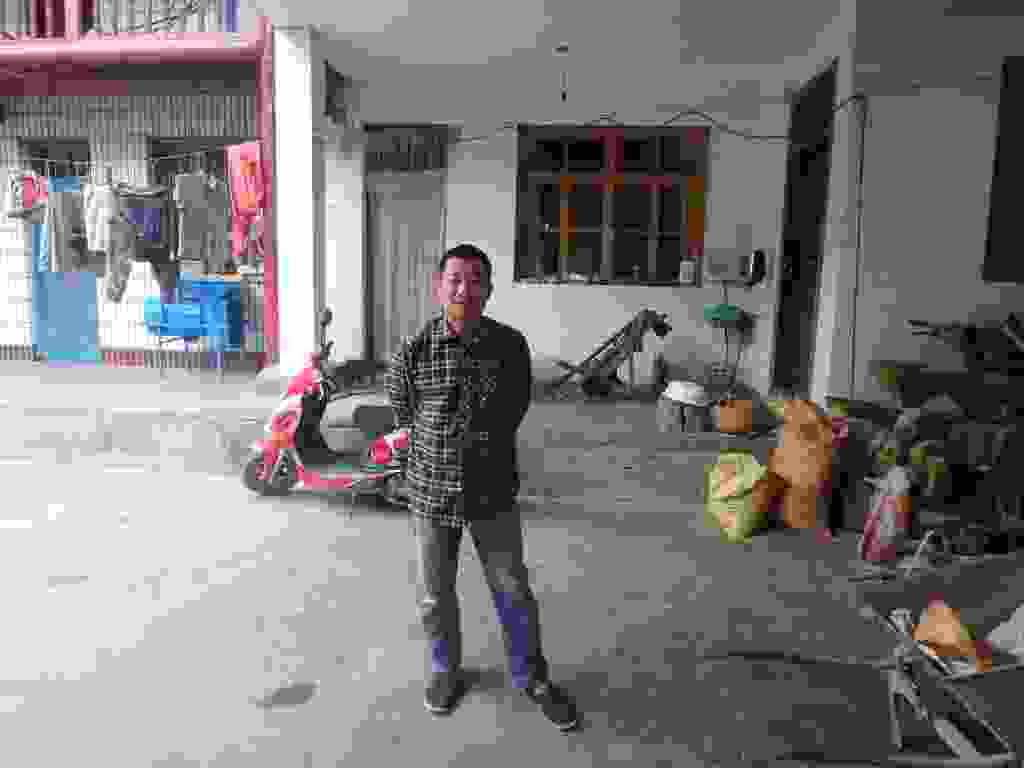
\includegraphics[width=\mywidth]{../wp-content/uploads/2015/09/wpid-p9136835-1024x768.jpg} } 
 \newline
 Les enfants sont tout fous quand je leur montre les photos que je prends d'eux \newline
 \newline
\centerline{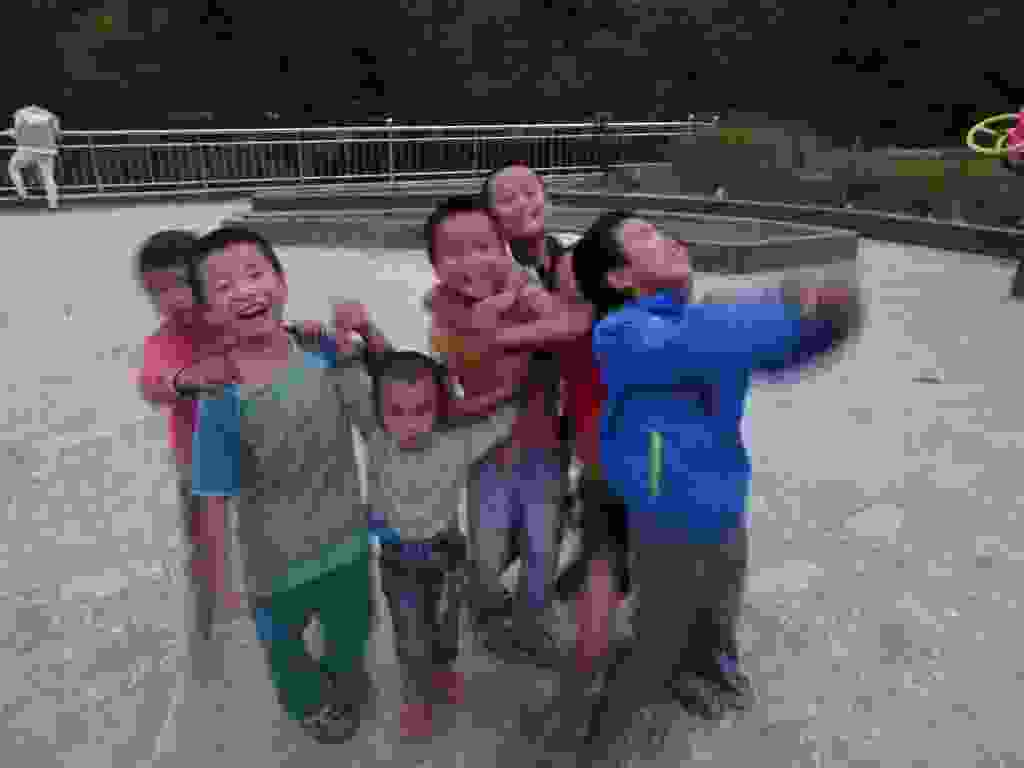
\includegraphics[width=\mywidth]{../wp-content/uploads/2015/09/wpid-p9126823-1024x768.jpg} } 
 \newline
 \newline
\centerline{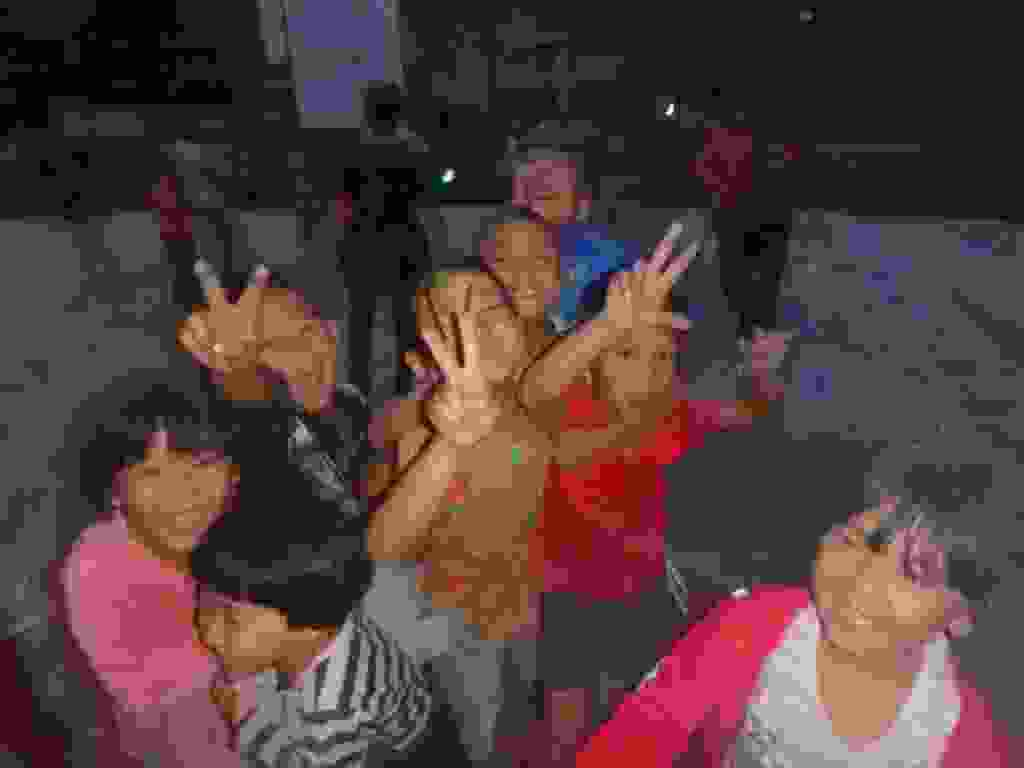
\includegraphics[width=\mywidth]{../wp-content/uploads/2015/09/wpid-p9126826-1024x768.jpg} } 
 \newline
 Malgré la communication difficile, je suis bien accueilli dans les restaurants et parfois on refuse de me faire payer l'addition \newline
 \newline
\centerline{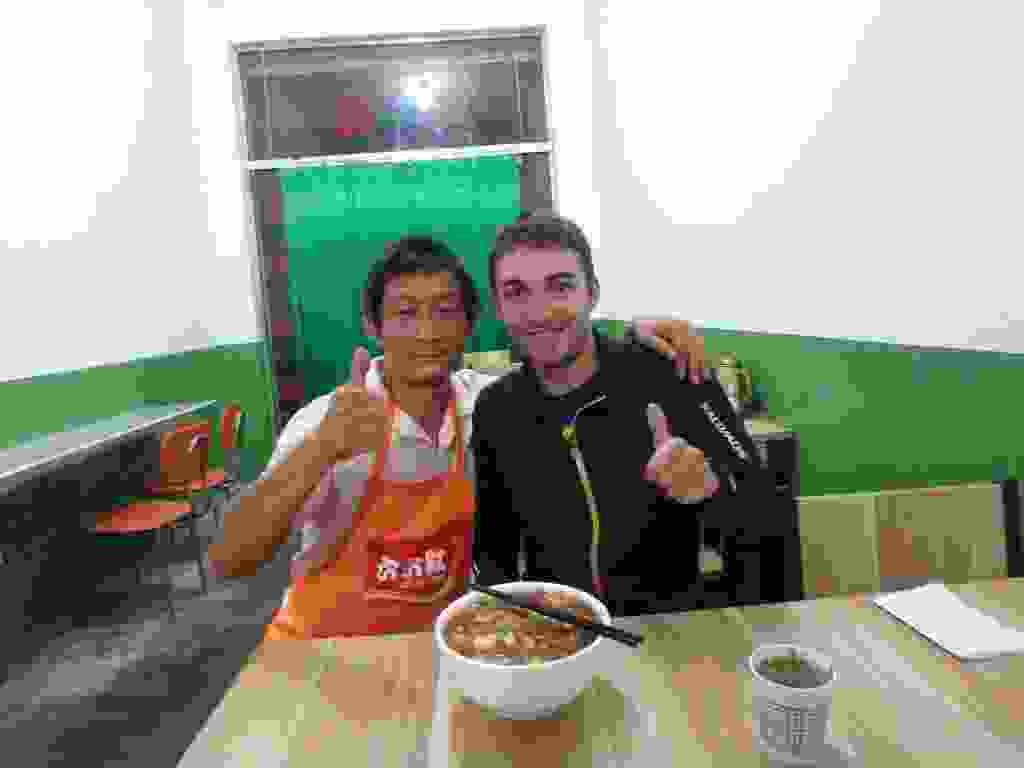
\includegraphics[width=\mywidth]{../wp-content/uploads/2015/09/wpid-p9096774-1024x768.jpg} } 
 \newline
 \newline
\centerline{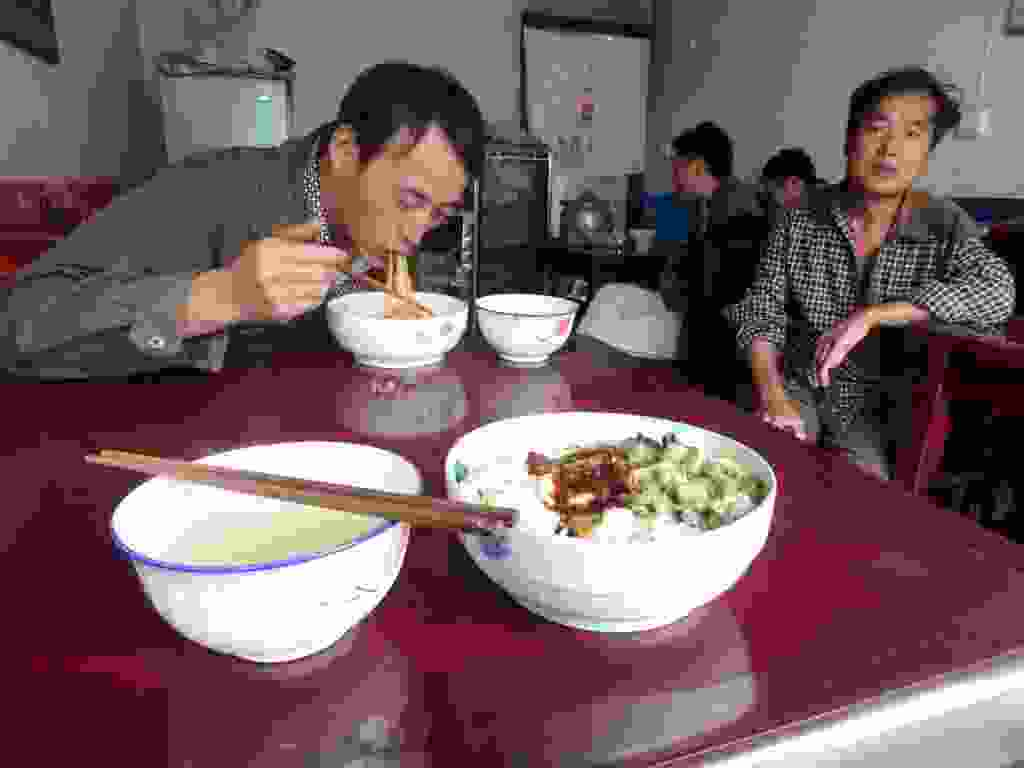
\includegraphics[width=\mywidth]{../wp-content/uploads/2015/09/wpid-p9096762-1024x768.jpg} } 
 \newline
 Les cols deviennent de plus en plus long en approchant de Jiuzhaigou \newline
 \newline
\centerline{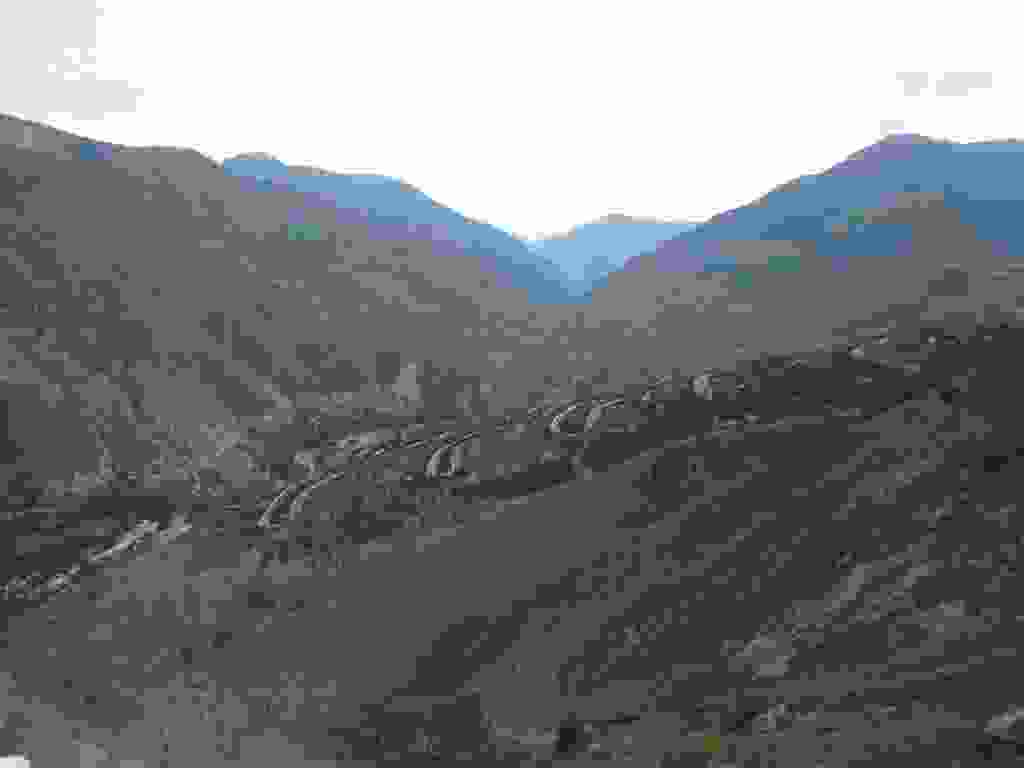
\includegraphics[width=\mywidth]{../wp-content/uploads/2015/09/wpid-p9136840-1024x768.jpg} } 
 \newline
 \newline
\centerline{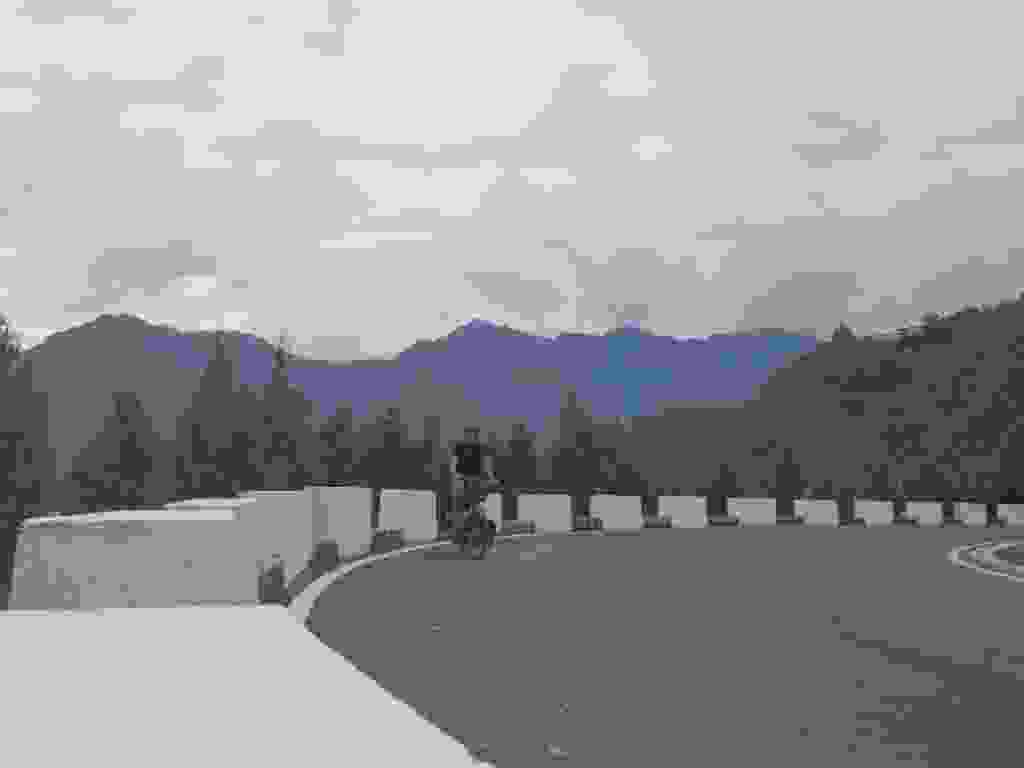
\includegraphics[width=\mywidth]{../wp-content/uploads/2015/09/wpid-p9136842-1024x768.jpg} } 
 \newline
 \newline
\centerline{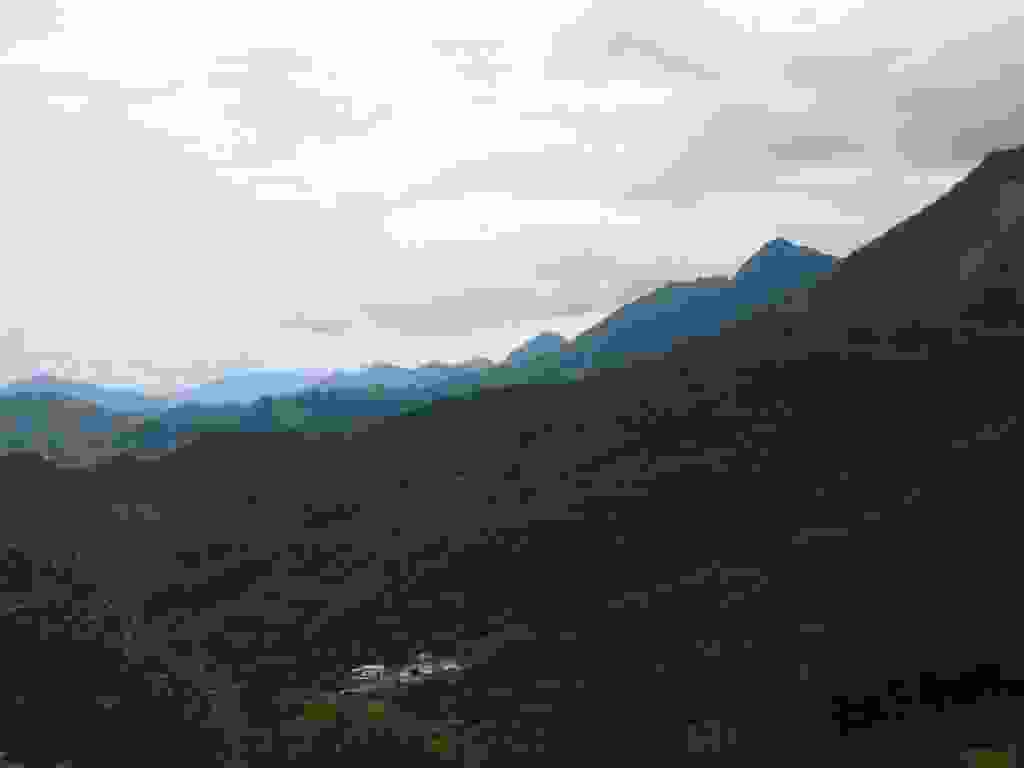
\includegraphics[width=\mywidth]{../wp-content/uploads/2015/09/wpid-p9136850-1024x768.jpg} } 
 \newline
 \newline
\centerline{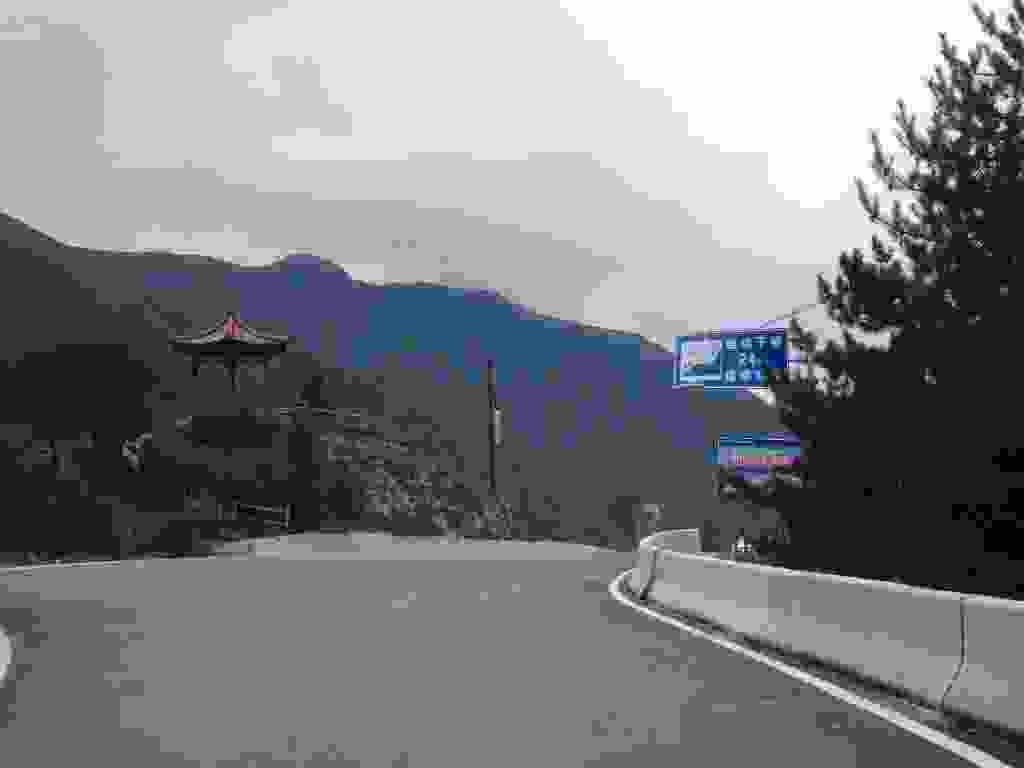
\includegraphics[width=\mywidth]{../wp-content/uploads/2015/09/wpid-p9136854-1024x768.jpg} } 
 \newline
 \newline
\centerline{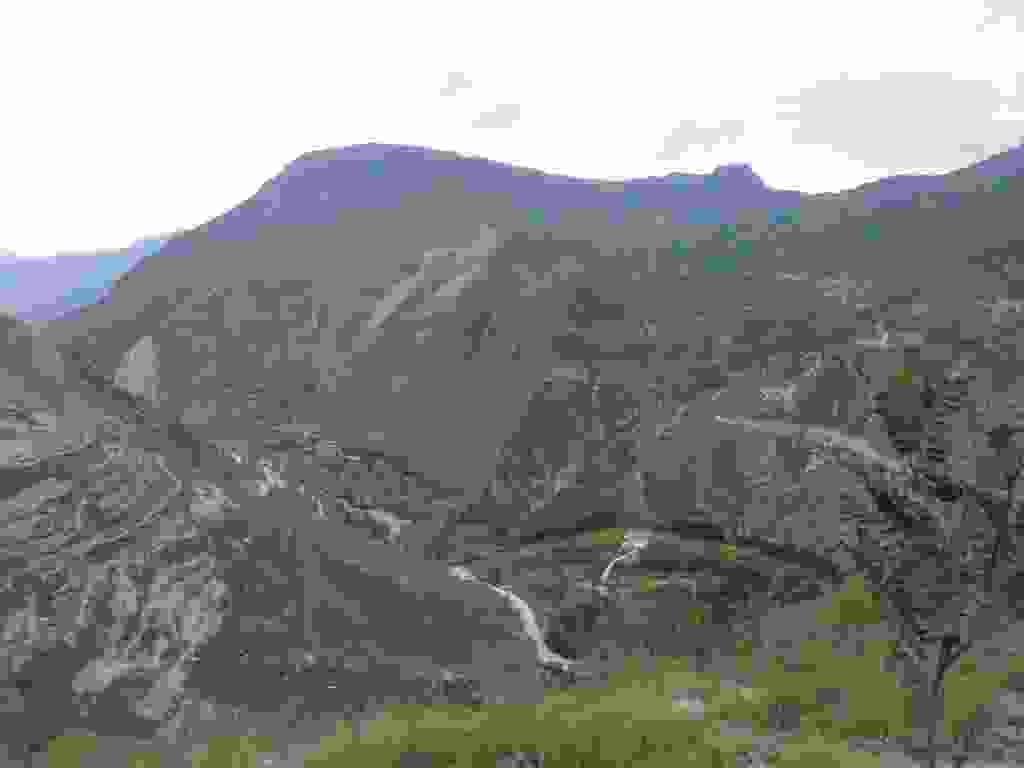
\includegraphics[width=\mywidth]{../wp-content/uploads/2015/09/wpid-p9136857-1024x768.jpg} } 
 \newline
 Le soleil fait son apparition le dernier jour \newline
 \newline
\centerline{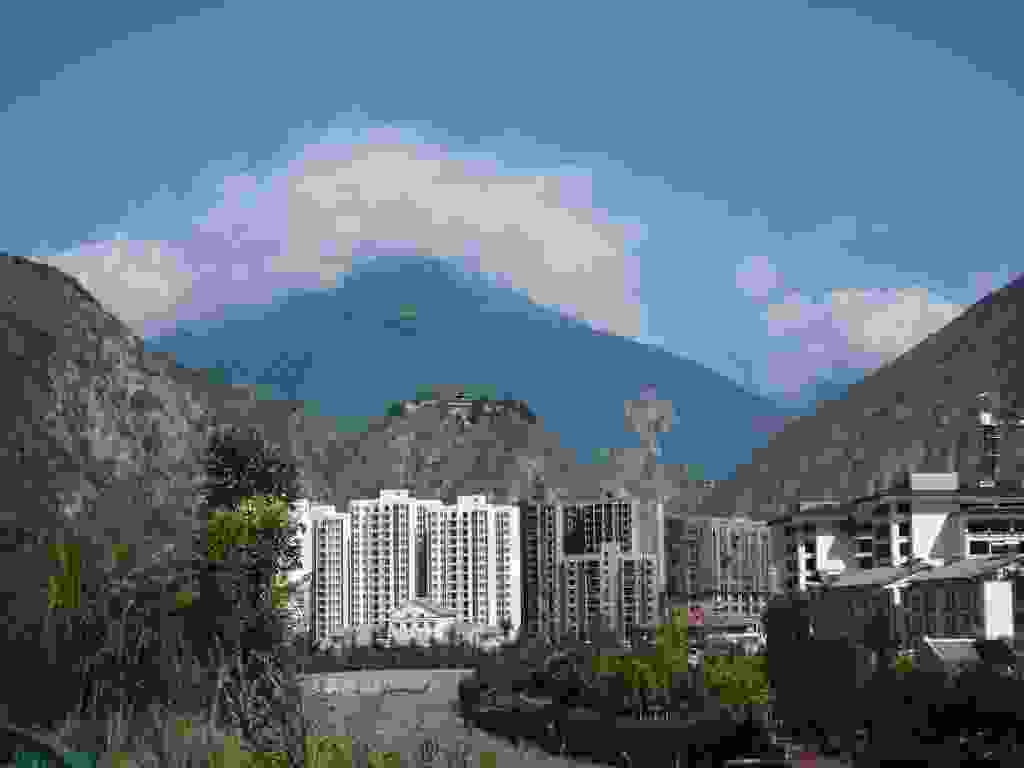
\includegraphics[width=\mywidth]{../wp-content/uploads/2015/09/wpid-p9146869-1024x768.jpg} } 
 \newline
 \newline
\centerline{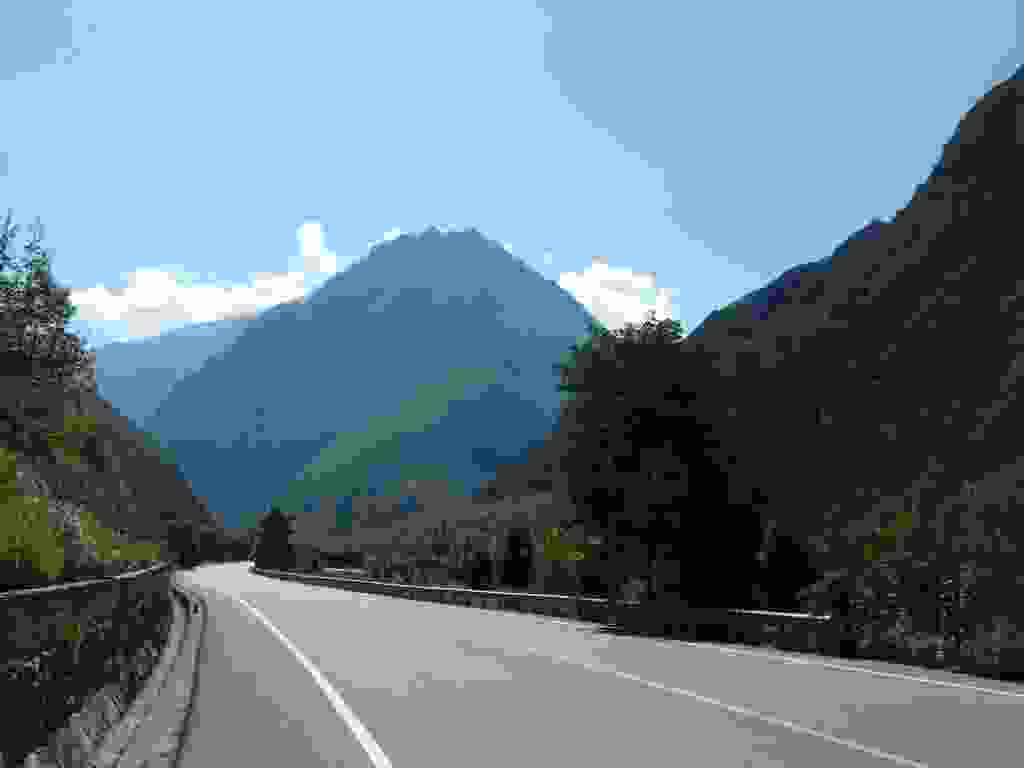
\includegraphics[width=\mywidth]{../wp-content/uploads/2015/09/wpid-p9146871-1024x768.jpg} } 
 \newline

\newpage
 
